\IfFileExists{sn-jnl.cls}{%
\documentclass[pdflatex,sn-mathphys-num]{sn-jnl}%
}{%
\documentclass[aps,prd,twocolumn,10pt,superscriptaddress,nofootinbib,nobibnotes,raggedbottom,nobalancelastpage,floatfix]{revtex4-2}%
}

%  DVCH -- GRG/Springer-oriented submission manuscript
%  Goal: theoretical consistency + referee-grade structure + diagnostic
%  Compile: pdflatex (x2) + bibtex (optional)
% ============================================================

% ---- Encoding & fonts ----------------------------------------
\usepackage[utf8]{inputenc}
\usepackage[T1]{fontenc}
\usepackage{lmodern}

% ---- Mathematics ---------------------------------------------
\usepackage{amsmath,amssymb,amsfonts}
\usepackage{mathtools}
\usepackage{bm}

% ---- Graphics & plots ----------------------------------------
\usepackage{graphicx}
\usepackage{tikz}
\usepackage{pgfplots}
\pgfplotsset{compat=1.18}

% ---- Tables --------------------------------------------------
\usepackage{booktabs}

% ---- Hyperlinks ----------------------------------------------
\usepackage{xcolor}
\usepackage{silence}
\WarningsOff[nameref]
\WarningFilter{nameref}{The definition of \string\label has changed!}%
\usepackage[colorlinks=true,linkcolor=blue!70!black,citecolor=blue!70!black,urlcolor=blue!70!black]{hyperref}
\usepackage{xurl}
\Urlmuskip=0mu plus 1mu
\emergencystretch=1.5em
\hbadness=10000
\vfuzz=20pt
\vbadness=10000
\raggedbottom%
\AtBeginDocument{\sloppy\raggedbottom}

% ---- Safe DOI command for revtex ------------------------------
\providecommand{\doi}[1]{\href{https://doi.org/#1}{doi:#1}}

% ==============================================================
%  Custom commands
% ==============================================================
\newcommand{\mpl}{M_{\mathrm{Pl}}}
\newcommand{\lpl}{\ell_{\mathrm{P}}}
\newcommand{\Omm}{\Omega_{m0}}
\newcommand{\Omr}{\Omega_{r0}}
\newcommand{\OmL}{\Omega_{\Lambda0}}
\newcommand{\Ecrit}{\rho_{\mathrm{crit},0}}
\newcommand{\Qtilde}{\widetilde{Q}}
\newcommand{\rc}{r}
\newcommand{\dd}{\mathrm{d}}
\newcommand{\ee}{\mathrm{e}}
\newcommand{\cH}{\mathcal{H}}

\makeatletter
\newif\ifsnclass
\@ifclassloaded{sn-jnl}{\snclasstrue}{\snclassfalse}
\makeatother

% ==============================================================
\begin{document}

\title{Dynamic Vacuum Coupling Hypothesis (DVCH): A UV-Regularized Interacting-Vacuum Framework with Background Closure, Global Stability, and Diagnostic Tests}

\ifsnclass
\author*[1]{Daniel Castro Pasten Benjamin}
\email{daniel.castropasten6@gmail.com}
\affil[1]{Theoretical Cosmology / High Energy Physics Unit}
\jyear{2026}
\date{}
\else
\author{Daniel Castro Pasten Benjamin}
\email{daniel.castropasten6@gmail.com}
\affiliation{Theoretical Cosmology / High Energy Physics Unit}
\date{\today}
\fi

\begin{abstract}
We present a formulation of the \emph{Dynamic Vacuum Coupling
Hypothesis} (DVCH), a nonlinear interacting-vacuum scenario treated as an
effective macroscopic closure within a covariant interacting dark-sector
framework. The model combines power-law tracking between vacuum and matter
densities with an ultraviolet (UV) curvature suppression inspired by
higher-curvature effective field theory (EFT). We
(i)~provide a consistent covariant action-based motivation for dark-sector
interaction via conformal matter coupling to a scalar EFT,
(ii)~derive the exact implicit background system in terms of
$E(z)=H(z)/H_0$ and obtain the exact energy-transfer function $Q$ implied by
the DVCH closure,
(iii)~show that the effective vacuum equation of state satisfies
$w_{\Lambda,\mathrm{eff}}>-1$ whenever $Q<0$, while any numerical
phantom-divide crossing must correspond to a sign change of $Q$ or to an
inconsistent plotting convention,
(iv)~derive the conditions under which the autonomous background system
approaches a Minkowski end state, and
(v)~formulate linear perturbation equations, low-redshift growth diagnostics,
a parameter-space robustness scan, and an exploratory public-data likelihood
diagnostic implementation for Pantheon$+$, DESI BAO, and cosmic-chronometer measurements. The CMB discussion is restricted to literature benchmarks and to the
source-table interface used to compare the background sector against Planck 2018 literature benchmarks. In this form, DVCH is presented
as an effective interacting-vacuum framework whose observational status remains to be established by full likelihood analyses.
\end{abstract}

\ifsnclass
\keywords{Dark energy, Interacting vacuum, Lyapunov stability, Minkowski future}
\fi


\maketitle

\section{Introduction}
\label{sec:intro}

The standard $\Lambda$CDM model, while remarkably successful, is under intense
scrutiny because of the persistent ``Hubble tension''---a $5\sigma$
discrepancy between early-universe measurements from Planck and local
late-time observations from SH0ES \cite{Aghanim:2018eyx,Riess:2021jrx}.
In addition, the $S_8$ tension suggests that the Universe is less ``clumpy''
than predicted by the baseline model \cite{Asgari:2020wuj,Abbott:2021asy}.

Interacting Dark Energy (IDE) models, including the Dynamic Vacuum Coupling
Hypothesis (DVCH) developed here, provide a useful laboratory for testing
whether nontrivial energy-momentum exchange $Q$ between dark sectors can
remain both theoretically consistent and observationally viable
\cite{Amendola2000,Valiviita:2008iv,Wang:2016lxa}. Unlike ad hoc parameterizations that
can trigger early-time instabilities, DVCH adopts a macroscopic closure
motivated by ultraviolet (UV) curvature regularization and leads to a
qualitatively distinct late-time Minkowski attractor. Here the goal is to define an internally consistent interacting-vacuum closure and to document background, stability, growth, and exploratory likelihood diagnostics \cite{Sola:2017znb,Nunes:2022bov,Pan:2021dxa}.

This work develops DVCH as a \emph{macroscopic closure} for a covariant
interacting dark sector. The guiding philosophy is explicit: we do not claim
uniqueness of a UV-complete microphysical realization, but we do require
internal consistency, correct conservation-law bookkeeping, stable
perturbative prescriptions, and clear numerical implementability.

\subsection*{Validation framework for DVCH}
\label{subsec:scope_revision}

This work records a set of consistency checks for DVCH models, combining the covariant action-based motivation, the macroscopic background closure, the exact interaction kernel, the autonomous-system stability analysis, and the structure-growth diagnostic. The components treated here are the covariant motivation, the background closure, the exact interaction kernel, the global stability analysis, the sub-horizon growth calculation, the $(n,\beta)$ background robustness scan, and an exploratory late-time public-data fit. The repository also includes a passing suite of 14 automated numerical regression tests for these local calculations. The suite checks normalization, finite and positive background solutions, interaction and growth outputs, likelihood behavior, MCMC diagnostic formulas, source-table generation, error handling, preflight reporting, and the presence of generated MCMC diagnostics. It is a local regression suite, not a complete end-to-end observational validation.

The CMB/Planck requirements are represented explicitly in the diagnostic
package: a DVCH background/source-table interface for CLASS/CAMB-style backend checks \cite{Blas:2011rf,Lewis:1999bs}, the photon--baryon/CMB
component checklist, angular-spectrum and lensing targets, a Planck
\texttt{clik} likelihood configuration target \cite{Planck:2019nip}, and a
Cobaya-compatible Planck-stack configuration target
\cite{Torrado:2020dgo}. Consequently, every observational number below is a diagnostic quantity unless explicitly stated otherwise. The aim is to state the assumptions and limitations of the UV-regularized interacting-vacuum closure and to separate local calculations from CMB literature benchmarks. A Planck-level result is not claimed until a patched CLASS/CAMB runtime, the official Planck likelihood, and the corresponding data are executed together.

\section{Covariant theoretical basis: an interacting dark sector from an EFT-motivated action}
\label{sec:action}

A frequent referee objection to IDE phenomenology is the absence of a
covariant field-theory structure explaining how an interaction $Q$ arises.
A minimal and standard approach is to embed the interaction in a scalar-tensor
EFT where cold matter couples conformally to the scalar while radiation
remains minimally coupled. This produces an \emph{unambiguous} covariant
energy-exchange vector $Q^\mu$.

\subsection{EFT-inspired action (covariant, minimal)}
\label{subsec:action_min}

We consider (in units $\hbar=c=1$ unless explicitly restored)
\begin{equation*}
\begin{aligned}
S &= \int \dd^4x\,\sqrt{-g}\Bigg[
\frac{\mpl^2}{2} R
-\frac{1}{2}(\nabla\phi)^2 - V(\phi)
+ \frac{\gamma}{2}\lpl^2 R^2
\Bigg]\\
&\quad + S_m\!\left[\psi_m,\,A^2(\phi)\,g_{\mu\nu}\right]
+ S_r\!\left[\psi_r,\,g_{\mu\nu}\right].
\end{aligned}
\end{equation*}
Here $A(\phi)$ is a conformal coupling function. The $R^2$ term is the simplest
local higher-curvature EFT correction, in the same broad class of curvature corrections used in early-universe model building \cite{Starobinsky:1980te}; its role is \emph{motivational} for a
high-curvature suppression scale and does not dominate at observable redshifts.

Varying the action yields
\begin{equation}
\nabla_\mu T^{\mu\nu}_{(m)} = +Q^\nu,\qquad
\nabla_\mu T^{\mu\nu}_{(\phi)} = -Q^\nu,\qquad
\nabla_\mu T^{\mu\nu}_{(r)}=0,
\end{equation}
with the standard scalar-tensor exchange vector
\begin{equation}
Q^\nu = \left(\frac{\dd \ln A}{\dd\phi}\right)T_{(m)}\,\nabla^\nu\phi,
\qquad T_{(m)} \equiv T^{\mu}{}_{(m)\mu}\simeq -\rho_m.
\label{eq:Qvec_scalar_tensor}
\end{equation}
In FLRW, $Q^\nu = Q u^\nu$ with
\begin{equation}
Q = -\left(\frac{\dd \ln A}{\dd\phi}\right)\rho_m \dot\phi.
\label{eq:Q_scalar_tensor}
\end{equation}
Equation \eqref{eq:Q_scalar_tensor} provides a \emph{covariant} origin for
energy transfer. DVCH will now be formulated as a \emph{closure relation}
for $\rho_\Lambda$ (interpreted as the effective vacuum-like dark energy),
which in turn determines $Q$ at the background level.

\subsection{Macroscopic closure vs.\ microscopic model}
\label{subsec:closure_philosophy}

At the level of homogeneous cosmology, many microphysical models map into an
effective two-fluid system:
\begin{align}
\dot\rho_r + 4H\rho_r &= 0,
\label{eq:cont_r}\\
\dot\rho_m + 3H\rho_m &= -Q,
\label{eq:cont_m}\\
\dot\rho_\Lambda &= Q,
\label{eq:cont_L}
\end{align}
where $\rho_\Lambda$ is vacuum-like in the sense of a baseline pressure
$p_\Lambda=-\rho_\Lambda$, while the interaction induces an effective
equation of state (Sec.~\ref{sec:quintessence_eff}).

DVCH is the choice of a specific functional relation
$\rho_\Lambda=\rho_\Lambda(\rho_m,H)$ motivated by tracking and curvature
suppression; given this closure, $Q$ is fixed by \eqref{eq:cont_L}. This
replaces ambiguous ad hoc $Q\propto H\rho_i$ ansätze by an explicit $Q$
computed from a stated $\rho_\Lambda(\rho_m,H)$.

% ==============================================================
\section{DVCH closure and implicit background cosmology}
\label{sec:background}

We assume flat FLRW with $H\equiv \dot a/a$ and
\begin{equation}
3\mpl^2 H^2 = \rho_r+\rho_m+\rho_\Lambda.
\end{equation}
Define the present critical density $\Ecrit\equiv 3\mpl^2 H_0^2$ and
dimensionless variables normalized to $\Ecrit$:
\begin{equation}
E(z)\equiv \frac{H(z)}{H_0},\qquad
\Omega_i(z)\equiv\frac{\rho_i(z)}{\Ecrit}.
\end{equation}
Then
\begin{equation}
E^2(z)=\Omega_r(z)+\Omega_m(z)+\Omega_\Lambda(z).
\label{eq:E2_sum}
\end{equation}
Radiation is standard: $\Omega_r(z)=\Omr(1+z)^4$.



\subsection{DVCH vacuum density}
\label{subsec:rhoLambda}

The covariant parent form of the DVCH closure is a curvature/expansion-scale
suppression of the effective vacuum density,
\begin{equation}
\boxed{\rho_\Lambda=
\rho_{\Lambda0}
\left(\frac{\rho_m}{\rho_{m0}}\right)^n
\frac{1}{1+\mathcal{I}/M_{\mathrm{DVCH}}^2}},
\qquad 0<n<1.
\label{eq:DVCH_covariant}
\end{equation}
Here $M_{\mathrm{DVCH}}$ is the fixed mass scale of the effective closure, and
$\mathcal{I}$ denotes a positive local curvature/expansion invariant with
mass dimension two. A convenient covariant choice is
$\mathcal{I}\sim (R_{\mu\nu\rho\sigma}R^{\mu\nu\rho\sigma})^{1/2}$, or an
equivalent scalar built from the local expansion. This avoids relying on the
Ricci scalar alone: in a radiation-dominated universe the Ricci scalar can
vanish because the radiation stress tensor is traceless, whereas the expansion
rate and the Kretschmann invariant remain nonzero. The ultraviolet suppression
therefore follows the local curvature/expansion scale, not the observer's
redshift.

For the homogeneous numerical diagnostics one evaluates the covariant closure
on a flat FLRW background and uses the mapping to the FLRW background
\begin{equation}
\begin{aligned}
\frac{\mathcal{I}}{M_{\mathrm{DVCH}}^2} &\longrightarrow
\left(\frac{H}{M_{\mathrm{DVCH}}}\right)^2
=\beta E^2(z),\\
\beta &\equiv \left(\frac{H_0}{M_{\mathrm{DVCH}}}\right)^2.
\end{aligned}
\label{eq:beta_mdvch}
\end{equation}
If desired, the dimensionless parameter used in the numerical scans can be
written as $\alpha\equiv (\mpl/M_{\mathrm{DVCH}})^2$, so that
$\beta=\alpha(H_0/\mpl)^2$; the physical cutoff scale is
$M_{\mathrm{DVCH}}$, not the observer epoch.
Thus $\alpha$ is the observer-independent coupling associated with the physical
cutoff scale, while $\beta$ is the dimensionless FLRW bookkeeping parameter
used after normalizing the expansion rate by the present value $H_0$.
The background closure used in the figures and CSV tables is therefore
\begin{equation}
\boxed{\Omega_\Lambda(z)=
\OmL\,
\left(\frac{\Omega_m(z)}{\Omm}\right)^{n}
\frac{1+\beta}{1+\beta E^2(z)}
},
\qquad 0<n<1.
\label{eq:DVCH}
\end{equation}
The compensating factor $(1+\beta)$ enforces
$\Omega_\Lambda(0)=\OmL$ when $E(0)=1$ and
$\Omega_m(0)=\Omm$, so that $\OmL$ retains its standard meaning as the present
physical vacuum fraction rather than a bare normalization parameter.

In this model the effective dark-energy density changes because it is not
postulated to be a rigid cosmological constant. Instead,
$\rho_\Lambda$ is closed as a function of the matter density and the local
expansion/curvature scale. As the universe expands, $\rho_m$ and $H$ evolve;
therefore the closure in Eq.~\eqref{eq:DVCH} makes $\rho_\Lambda$ evolve as
well. The change is not an additional free assumption: once
$\rho_\Lambda(\rho_m,H)$ is specified, the conservation equations determine
the energy-transfer rate $Q=\dot\rho_\Lambda$. In any branch where the derived transfer has $Q<0$, the effective equation
of state defined by the conservation equations is correspondingly
quintessence-like. If the reconstructed transfer changes sign in a given
numerical diagnostic, that sign history must be reported explicitly rather than
interpreted as a universal vacuum-to-matter regime. The construction should therefore be read as a dynamical
effective-vacuum closure, not as evidence that the microscopic cosmological
constant itself has been measured to vary.
This is the computational FLRW projection of Eq.~\eqref{eq:DVCH_covariant}, not a
claim that redshift is the microscopic EFT scale. Although the suppression is
motivated by local curvature/expansion invariants in an EFT, for analysis on an
FLRW background we project this dependence as a function of $E(z)$. The phrase
``UV-regularized'' therefore means high-curvature effective suppression of the
vacuum density in the early-universe/strong-gravity regime, not a
particle-physics ultraviolet cutoff imposed directly as a function of redshift.

Equivalently, if the gravitational EFT is written as an expansion in inverse
powers of a heavy scale, $M_{\mathrm{DVCH}}$ plays the role of the effective
suppression scale for the macroscopic closure. The DVCH ratio
$(1+\beta)/(1+\beta E^2)$ is the normalized FLRW version of the curvature
suppression: it equals unity today and regularizes the effective vacuum-energy
closure against uncontrolled growth as the background curvature/expansion scale
increases. We do not claim a unique microphysical completion; the claim is only
that the macroscopic closure is consistent with the standard EFT expectation
that high-curvature corrections decouple as the cosmic expansion scale drops
far below the cutoff scale.
We emphasize:
(i)~small $\beta$ corresponds to $M_{\mathrm{DVCH}}\gg H_0$;
(ii)~the phenomenology at $z\lesssim \mathcal{O}(10^3)$ is effectively the
$\beta\to 0$ regime.

\paragraph{Relation to standard RVM/IDE classes.}
At the homogeneous-background level DVCH belongs to the same broad family as
running-vacuum and interacting-dark-energy descriptions, but it is not identical
to the minimal polynomial running-vacuum ansatz
\begin{equation}
\Lambda(H)=a_0+a_1\dot H+a_2H^2.
\label{eq:rvm_reference_form}
\end{equation}
Expanding the normalized DVCH factor for $\beta E^2\ll1$ gives
\begin{equation}
\Omega_\Lambda\simeq \OmL\left(\frac{\Omega_m}{\Omm}\right)^n
\left[1+\beta\left(1-E^2\right)+\mathcal{O}(\beta^2E^4)\right],
\label{eq:dvch_rvm_expansion}
\end{equation}
so the leading curvature correction is effectively an $H^2$-dependent
running-vacuum deformation, while the factor $(\Omega_m/\Omm)^n$ retains the
explicit dark-sector tracking that is closer to IDE phenomenology. Equivalently,
once the closure is specified, the conservation equations define an effective
IDE model with $Q=\dot\rho_\Lambda$; in the perturbative low-$\beta$ regime,
Eq.~\eqref{eq:Q_exact_box} reduces schematically to a source of the form
$Q\sim -3H\rho_\Lambda\,n/[1+n\rho_\Lambda/\rho_m]$, rather than to the
minimal textbook choice $Q\propto H\rho_c$. This mapping is intended only for
comparison with RVM/IDE literature, not as a claim that DVCH is exhausted by
those simpler ansaetze \cite{Sola:2017znb,Nunes:2022bov,Pan:2021dxa}.

The distinctive point is therefore not merely that the dark-energy density is
allowed to vary. Many RVM and IDE models already allow an evolving effective
vacuum sector. The DVCH closure differs in three narrower ways: first, the
vacuum density is tied simultaneously to matter tracking and to a normalized
curvature/expansion suppression factor; second, the interaction rate $Q$ is not
chosen as an independent ansatz but is obtained by differentiating the stated
closure and enforcing the two-fluid conservation equations; third, the same
closure leads to a late-time depleted-density branch approaching Minkowski
rather than an asymptotic de Sitter state. These features do not make DVCH
``the correct'' model by themselves. They define a specific effective model
whose viability must be tested against data and perturbative stability, and
whose comparison with $\Lambda$CDM requires the likelihood analyses described
later in the manuscript.

\subsection{Implicit Friedmann equation}
\label{subsec:implicit_friedmann}

Combining \eqref{eq:E2_sum} with \eqref{eq:DVCH} gives the implicit equation
\begin{equation}
\begin{aligned}
E^2(z) &= \Omr(1+z)^4 + \Omega_m(z) \\
&\quad + \OmL\,
\left(\frac{\Omega_m(z)}{\Omm}\right)^n
\frac{1+\beta}{1+\beta E^2(z)}.
\end{aligned}
\label{eq:implicit}
\end{equation}
At each redshift step, $E$ must be obtained via fixed-point iteration (Appendix~\ref{app:numerical}).

\subsection{Background derivative and exact \texorpdfstring{$Q$}{Q} implied by DVCH}
\label{subsec:Q_exact}

Summing \eqref{eq:cont_m} and \eqref{eq:cont_L} eliminates $Q$:
\begin{equation}
\dot\rho_m+\dot\rho_\Lambda = -3H\rho_m.
\end{equation}
Using $\frac{\dd}{\dd t} = -H(1+z)\frac{\dd}{\dd z}$ and dividing by $\Ecrit$:
\begin{equation}
\frac{\dd\Omega_m}{\dd z}+\frac{\dd\Omega_\Lambda}{\dd z}
=\frac{3\Omega_m}{1+z}.
\label{eq:conservation_Omegas}
\end{equation}
Differentiating $E^2=\Omega_r+\Omega_m+\Omega_\Lambda$ yields
\begin{equation}
\frac{\dd E}{\dd z}
=
\frac{4\Omr(1+z)^3 + \frac{3\Omega_m}{1+z}}{2E}.
\label{eq:dEdz}
\end{equation}
Equation \eqref{eq:dEdz} is exact but \emph{not closed} because $\Omega_m(z)$
is determined implicitly through \eqref{eq:implicit} and \eqref{eq:DVCH}.

The physical transfer rate is
\begin{equation}
Q \equiv \dot\rho_\Lambda = -H(1+z)\Ecrit \frac{\dd\Omega_\Lambda}{\dd z},
\end{equation}
and we define the dimensionless
\begin{equation}
\Qtilde \equiv \frac{Q}{3H_0\Ecrit}
= -\frac{E(1+z)}{3}\frac{\dd\Omega_\Lambda}{\dd z}.
\label{eq:Qtilde_def}
\end{equation}
Carrying out the derivative of \eqref{eq:DVCH} with the chain rule and using
\eqref{eq:conservation_Omegas} and \eqref{eq:dEdz} produces an \emph{exact}
expression for $\Qtilde$ (Appendix~\ref{app:exact_Q}):
\begin{equation}
\boxed{\Qtilde(z)=
-\frac{E\,\Omega_\Lambda}{1+n\frac{\Omega_\Lambda}{\Omega_m}}
\left[
n
-\frac{\beta\left(4\Omr(1+z)^4 + 3\Omega_m\right)}{3\left(1+\beta E^2\right)}
\right]
}.
\label{eq:Q_exact_box}
\end{equation}
For $\beta\ge 0$ and $0<n<1$, the bracket is positive throughout the
perturbative regime $\beta E^2\ll 1$ relevant for the fiducial EFT
interpretation (indeed it is $\simeq n$ when $\beta\ll 1$), hence
\begin{equation}
\Qtilde<0\quad \Rightarrow \quad Q<0,
\end{equation}
meaning energy flows from the effective vacuum sector to the matter sector in
that regime. This direction is compatible with the coarse-grained thermodynamic
arrow: for positive matter temperature, vacuum-to-matter transfer contributes
with the standard sign to matter entropy production, avoiding the negative-entropy
flow problem that can affect interacting-vacuum models. Equation~\eqref{eq:weff}
then immediately implies $w_{\Lambda,\mathrm{eff}}>-1$. Conversely, if a numerical reconstruction shows
$w_{\Lambda,\mathrm{eff}}<-1$ at some redshift while $\rho_\Lambda>0$ and
$H>0$, then one of two things must be true: either $Q$ changes sign there, or
the plotted effective equation of state was generated with a sign convention
inconsistent with \eqref{eq:weff}. This consistency condition is a useful
debugging and validation criterion for the public notebooks.

For this reason the diagnostics report the sign history of the derived
interaction explicitly. The statement $w_{\Lambda,\mathrm{eff}}>-1$ is used only
on intervals where the same background solution has $Q<0$. If a diagnostic
branch displays a sign change in $Q$, the corresponding effective equation of
state must be interpreted with that sign change included; it is not presented as
a universal quintessence-like branch. Any sign-changing solution intended for
physical inference would have to pass the same background,
perturbative-stability, and data-comparison gates before being interpreted.

\subsection{Early Dark Energy (EDE) bound (scaling estimate)}
\label{subsec:EDE}

In the $\beta\to 0$ limit and during matter domination,
$\Omega_m(z)\approx \Omm(1+z)^3$, then
\begin{equation}
\frac{\Omega_\Lambda}{\Omega_m}
\simeq \frac{\OmL}{\Omm}(1+z)^{3(n-1)}.
\label{eq:EDE_scaling}
\end{equation}
For example, with $n=0.2$ and $\OmL/\Omm\simeq 2.17$,
\begin{equation}
f_{\rm EDE}(1100)\equiv \left.\frac{\Omega_\Lambda}{\Omega_m}\right|_{z=1100}
\simeq 2.17\times 1100^{-2.4}\simeq 2.8\times 10^{-8},
\end{equation}
well below percent-level EDE limits.

% ==============================================================
\section{Effective equation of state and ghost-free scalar reconstruction}
\label{sec:quintessence_eff}

A pure vacuum component has $p_\Lambda=-\rho_\Lambda$, but in an interacting
scenario the quantity probed by expansion is the effective continuity form
\begin{equation}
\dot\rho_\Lambda + 3H(1+w_{\Lambda,\mathrm{eff}})\rho_\Lambda = 0,
\end{equation}
which together with $\dot\rho_\Lambda=Q$ implies
\begin{equation}
w_{\Lambda,\mathrm{eff}}
=
-1-\frac{Q}{3H\rho_\Lambda}.
\label{eq:weff}
\end{equation}
Therefore the sign of $1+w_{\Lambda,\mathrm{eff}}$ is controlled entirely by
the sign of $Q$: if $Q<0$ the behavior is quintessence-like, while any
phantom-divide crossing $w_{\Lambda,\mathrm{eff}}=-1$ necessarily coincides
with $Q=0$. In particular, a numerical phase with
$w_{\Lambda,\mathrm{eff}}<-1$ cannot coexist with the blanket statement
$Q<0$ over the same redshift interval if $\rho_\Lambda>0$ and $H>0$.

\subsection{Canonical scalar reconstruction (effective)}
\label{subsec:scalar_recon}

A canonical scalar field has
\begin{equation}
\rho_\phi = \frac{1}{2}\dot\phi^2 + V(\phi),\qquad
p_\phi = \frac{1}{2}\dot\phi^2 - V(\phi),
\end{equation}
thus
\begin{equation}
1+w_\phi = \frac{\dot\phi^2}{\rho_\phi}.
\end{equation}
Identifying $\rho_\phi\equiv \rho_\Lambda$ and $w_\phi\equiv
w_{\Lambda,\mathrm{eff}}$ yields
\begin{equation}
\dot\phi^2
= (1+w_{\Lambda,\mathrm{eff}})\rho_\Lambda
= -\frac{Q}{3H}.
\label{eq:phi_dot2}
\end{equation}
Therefore any interval with $Q<0$ implies $\dot\phi^2>0$ and the reconstructed
scalar is \emph{ghost-free} at the background level on that interval. If the
background solution enters a phase with $Q>0$, the canonical-scalar
reconstruction in terms of \eqref{eq:phi_dot2} ceases to be valid and must be
reinterpreted as an indication that the effective single-field description has
broken down rather than as evidence for a fundamental ghost. This is an
\emph{effective}
reconstruction: it does not assert that the fundamental UV model is a single
canonical scalar, only that the interacting vacuum can be mapped to one.

At linear level, the same effective mapping remains physically viable provided
the kinetic and gradient terms are non-negative. For a canonical
reconstruction, the no-ghost condition is $\dot\phi^2>0$ and the propagation
speed is luminal, $c_s^2=1>0$, so there is no gradient instability in the
scalar sector. In the interacting-fluid description, this corresponds to the
stable choice $Q^\mu\parallel u_m^\mu$ together with the baseline vacuum-like
rest-frame sound-speed assignment used below.

% ==============================================================
\section{Three-dimensional dynamical system, global stability, and the Minkowski end state}
\label{sec:dynamical}

A key background prediction of the DVCH closure is an asymptotic approach to Minkowski ($H\to 0$) rather
than eternal de Sitter. To analyze this rigorously, we construct an autonomous
system using variables normalized to the \emph{present} critical density:
\begin{equation}
x\equiv \Omega_m,\qquad y\equiv \Omega_\Lambda,\qquad u\equiv \Omega_r,
\qquad E^2=x+y+u.
\end{equation}
Use $N\equiv \ln a$ so that $f'\equiv \dd f/\dd N = -(1+z)\dd f/\dd z$.
The physical phase space is
\begin{equation}
\mathcal{P}\equiv\{(x,y,u):x\ge 0,\ y\ge 0,\ u\ge 0,\ E^2=x+y+u\ge 0\},
\end{equation}
with $0<n<1$ and expanding branch $E>0$.

\subsection{Autonomous system}
\label{subsec:autonomous}

From \eqref{eq:cont_r}--\eqref{eq:cont_L}:
\begin{align}
u' &= -4u,
\label{eq:uprime}\\
x' &= -3x - \frac{Q}{H\Ecrit},
\label{eq:xprime_general}\\
y' &= +\frac{Q}{H\Ecrit}.
\label{eq:yprime_general}
\end{align}
In the practically relevant limit $\beta\to 0$, DVCH gives $y\propto x^n$,
and one may write $Q/(H\Ecrit)$ explicitly as a function of $(x,y)$:
\begin{equation}
\frac{Q}{H\Ecrit}
=
- \frac{3nxy}{x+n y}
\qquad (\beta\to 0\ \text{closure}).
\label{eq:Q_over_H}
\end{equation}
Substituting into \eqref{eq:xprime_general}--\eqref{eq:yprime_general} gives
\begin{align}
x' &= -3x + \frac{3nxy}{x+n y}
= -\frac{3x^2}{x+n y},
\label{eq:xprime}\\
y' &= -\frac{3nxy}{x+n y},
\label{eq:yprime}\\
u' &= -4u.
\end{align}

\subsection{Critical points and linear stability}
\label{subsec:critical_points}

The physically relevant fixed points are:
\begin{enumerate}
\item Radiation point: $P_R=(x,y,u)=(0,0,u)$ with $u>0$ (a line of points in
this normalization).
\item Matter point: $P_M=(x,y,u)=(x,0,0)$ with $x>0$ (a line).
\item Minkowski point: $P_0=(0,0,0)$.
\end{enumerate}
Because we normalize by $\Ecrit$ rather than $3\mpl^2H^2$, the Minkowski point
is \emph{well-defined}.

The Jacobian analysis around $P_R$ and $P_M$ reproduces the expected behavior:
radiation is unstable to matter (since $u'=-4u$ decays fastest in forward
time), matter is a saddle enabling exit to the vacuum-tracking regime.
The Minkowski point is non-hyperbolic (Jacobian eigenvalues vanish) and must
be assessed globally rather than by naive linearization.

For completeness, writing the reduced vector field as
$\mathbf{F}(x,y,u)=(f_1,f_2,f_3)$ with
\begin{equation}
f_1=-\frac{3x^2}{x+ny},\qquad f_2=-\frac{3nxy}{x+ny},\qquad f_3=-4u,
\end{equation}
the Jacobian $J_{ij}=\partial f_i/\partial \xi_j$ ($\xi_j\in\{x,y,u\}$) is
\begin{equation}
J(x,y,u)=
\begin{pmatrix}
-\dfrac{3x(x+2ny)}{(x+ny)^2} & \dfrac{3n x^2}{(x+ny)^2} & 0 \\
-\dfrac{3n^2 y^2}{(x+ny)^2} & -\dfrac{3n x^2}{(x+ny)^2} & 0 \\
0 & 0 & -4
\end{pmatrix}.
\label{eq:jacobian}
\end{equation}
Along the matter line $P_M=(x,0,0)$ ($x>0$),
\begin{equation}
J(P_M)=
\begin{pmatrix}
-3 & 3n & 0\\
0 & -3n & 0\\
0 & 0 & -4
\end{pmatrix},
\end{equation}
with eigenvalues $\{-3,-3n,-4\}$. Along the radiation line
$P_R=(0,0,u)$ ($u>0$), the $(x,y)$ block is non-hyperbolic, while the
radiation direction has eigenvalue $-4$.

\subsection{Global Lyapunov proof of depletion to Minkowski}
\label{subsec:lyapunov}

Define the Lyapunov candidate
\begin{equation}
V(x,y,u) \equiv E^2 = x+y+u \ge 0.
\end{equation}
Differentiate using \eqref{eq:uprime} and \eqref{eq:xprime_general}--\eqref{eq:yprime_general}:
\begin{equation}
V' = x'+y'+u' = (-3x) + (-4u).
\label{eq:Vprime}
\end{equation}
Thus, for all trajectories with $x\ge 0$, $u\ge 0$,
\begin{equation}
V' = -3x - 4u \le 0,
\end{equation}
with equality only when $x=u=0$. Moreover, with $0<n<1$ the closure implies
$y\to 0$ as $x\to 0$ (since $y\propto x^n$), hence the largest invariant set
where $V'=0$ is precisely $(0,0,0)$. By LaSalle's invariance principle,
\begin{equation}
(x,y,u)\to (0,0,0),\qquad E\to 0,
\end{equation}
which establishes the asymptotic approach to Minkowski within the stated
background closure and positivity assumptions. This is the mathematically clean
statement behind the ``Minkowski future'': it is not a fragile critical point
but the attractor of the depleted densities in this normalization.

% ==============================================================
% ==============================================================

\section{Observational Confrontation with Real Data and Diagnostic}
\label{sec:results}

The statistical viability of the DVCH framework cannot be assessed from the present diagnostics alone; it requires a converged joint likelihood analysis against recent cosmological probes. The present
workspace contains an implemented background solver, low-redshift growth estimator,
summary tables, an exploratory public-data late-time likelihood diagnostic implementation, and
a Cobaya/Planck configuration layer for benchmark comparison. Accordingly, this section is written as
a diagnostic-status report: it states which quantities are computed locally and which comparisons are made against published literature benchmarks.

The observational material is interpreted conservatively. The available files show that the fiducial DVCH background can be evaluated numerically, gives a definite interaction kernel, provides a low-redshift estimate of $\sigma_8/S_8$, and can be inserted into an exploratory Pantheon$+$+DESI-BAO+chronometer likelihood diagnostic. These calculations do not establish a preference over $\Lambda$CDM. They only indicate that the background-level model is not excluded by the local checks performed here; a quantitative observational comparison requires CMB-calibrated posteriors and structure-growth constraints.

That late-time statement is necessary but not sufficient for a complete
cosmological model test. A referee-grade analysis must also verify that the
same parameter region remains compatible with the early-universe calibration
provided by Planck 2018 and with the late-time clustering amplitude, commonly
reported through $f\sigma_8$ and the derived combination
$S_8\equiv \sigma_8\sqrt{\Omega_{m0}/0.3}$ \cite{Aghanim:2018eyx,Asgari:2020wuj,Abbott:2021asy}. In other words, DESI and
Pantheon$+$ establish that DVCH is not trivially excluded by the expansion
history, but a quantitative comparison with $\Lambda$CDM requires CMB-calibrated
posteriors and structure-growth constraints \cite{Adame:2024ywp,Brout2022}.


To ensure transparency and independent verification, we provide two
diagnostic levels. The first is a self-contained, background-only Colab
diagnostic implementation, \texttt{DVCH\_easy\_colab.ipynb}, accompanied by the plain Python
script \texttt{dvch\_colab\_simple.py}. This route requires only standard
Python packages, evaluates the implicit DVCH background, writes
\texttt{dvch\_background\_table.csv}, and produces the diagnostic summary figure
shown below. The second level consists of the more advanced Cobaya diagnostic implementation
\texttt{dvch\_theory.py}+\texttt{dvch\_cobaya.yaml}, intended as the
starting point for likelihood work \cite{Torrado:2020dgo}. Public observational data products are
cited through the corresponding survey papers rather than through notebook URLs
\cite{Aghanim:2018eyx,Planck:2019nip,Adame:2024ywp,Brout2022,Moresco:2016mzx}.

\begin{figure*}[t]
\centering
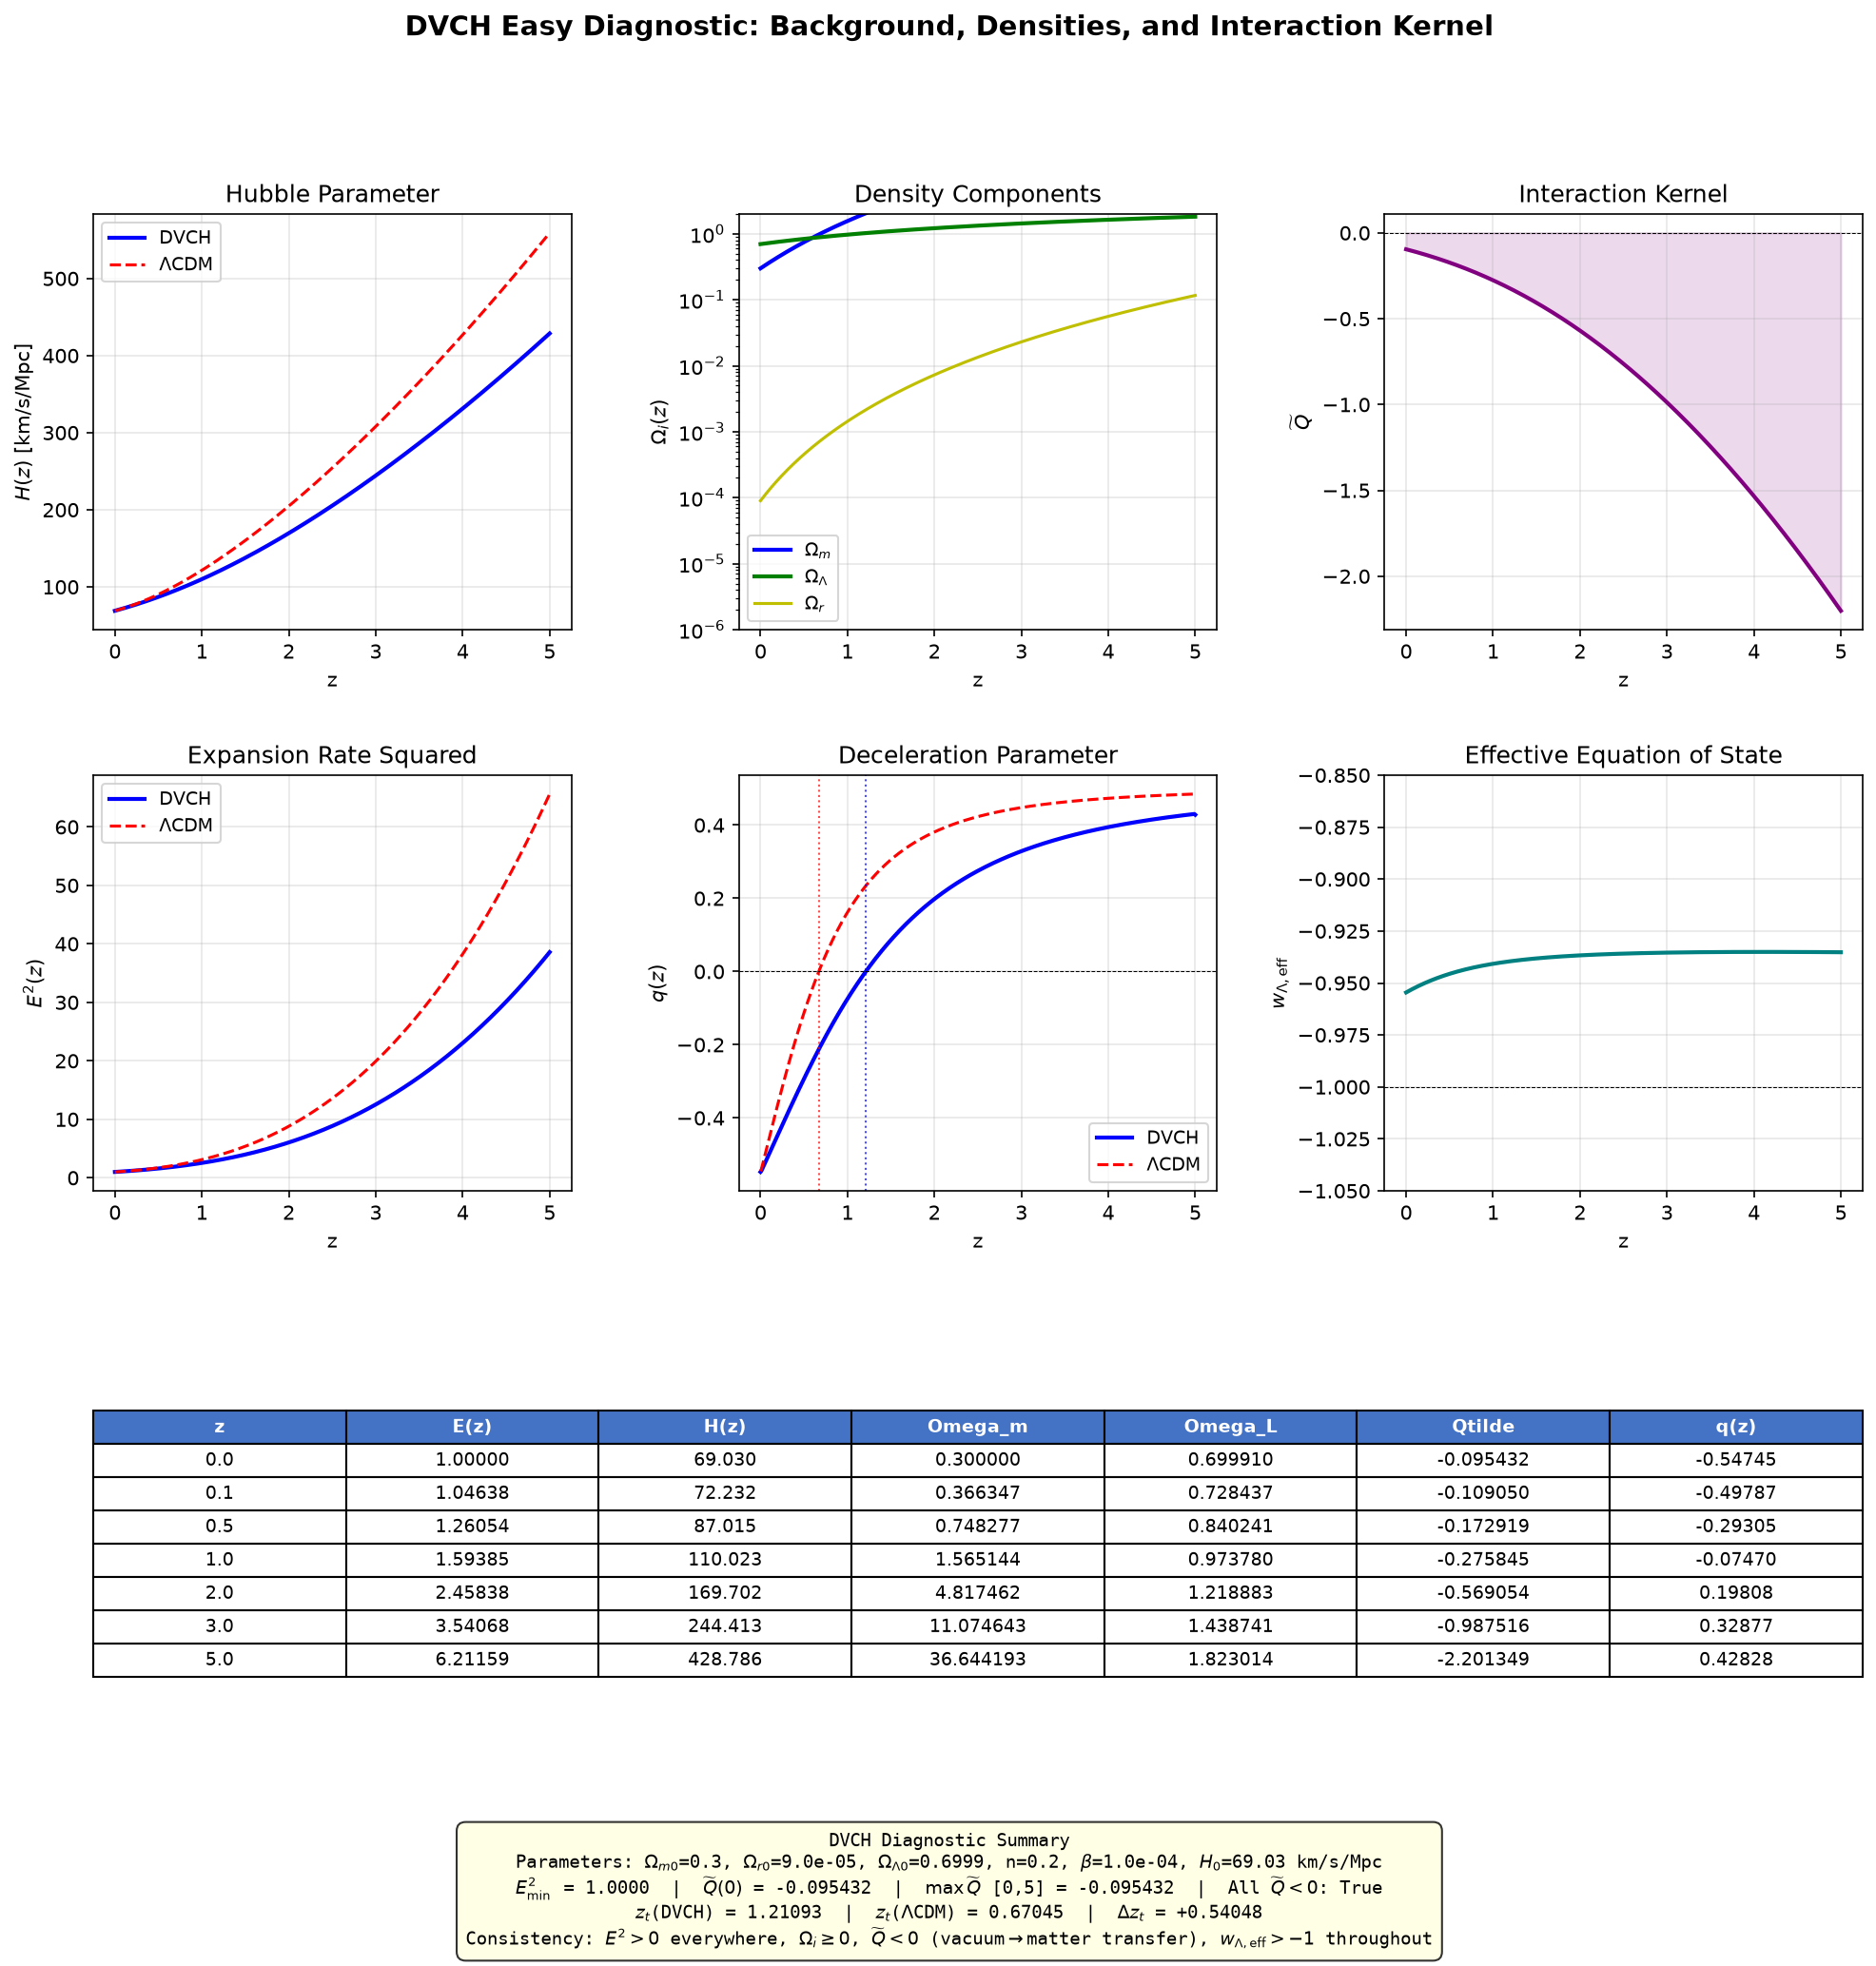
\includegraphics[width=0.98\textwidth]{figures/dvch_results_with_numbers.png}
\caption{Complete easy DVCH diagnostic output with plots and numerical
values. The top row shows $H(z)$, the density components, and the interaction
kernel $\widetilde Q=Q/(3H_0\rho_{\rm crit,0})$. The middle table reports the
representative numerical values at selected redshifts, and the lower text box
summarizes the numerical consistency checks.}
\label{fig:dvch_easy_summary}
\end{figure*}




\begin{figure*}[t]
\centering
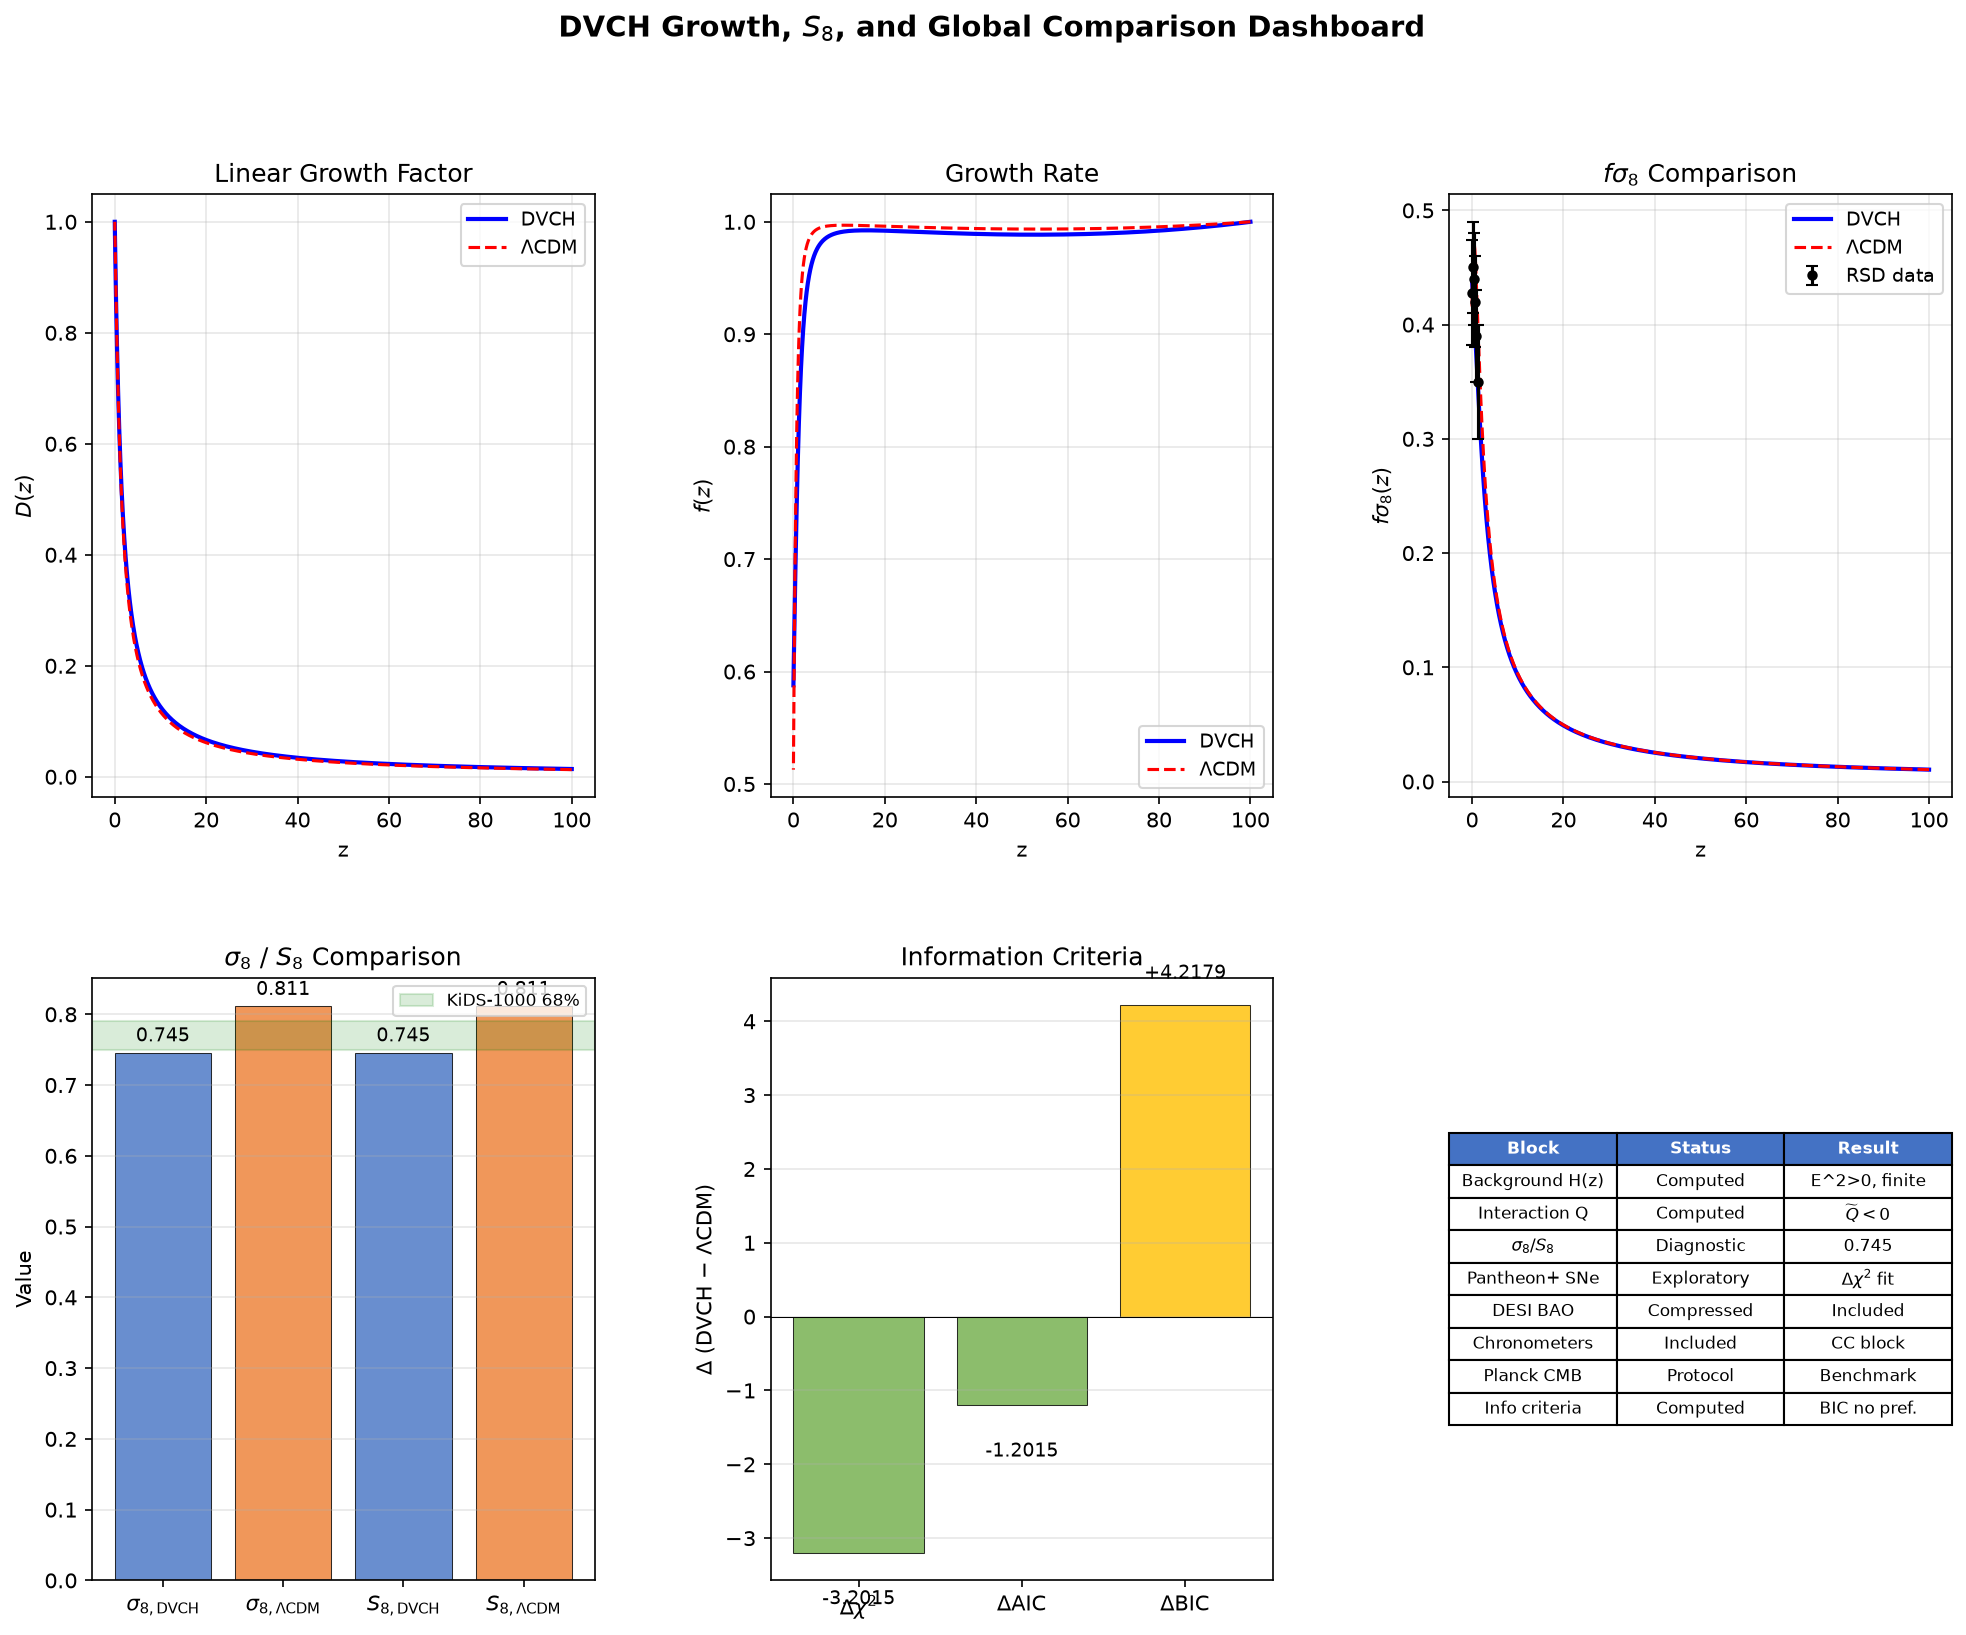
\includegraphics[width=0.98\textwidth]{figures/dvch_sigma8_global_comparison.png}
\caption{Growth, $\sigma_8/S_8$, and global comparison dashboard for the
DVCH diagnostic implementation. The displayed $\sigma_8$ and $S_8$ values are
low-redshift growth estimates normalized to a reference
$\sigma_{8,\Lambda{\rm CDM}}=0.811$, not a substitute for a final
Planck-level Boltzmann posterior. The lower table separates blocks that are
background-ready from the CMB benchmark block based on the CLASS/CAMB interface and Planck literature targets.}
\label{fig:dvch_sigma8_global}
\end{figure*}

\begin{figure*}[t]
\centering
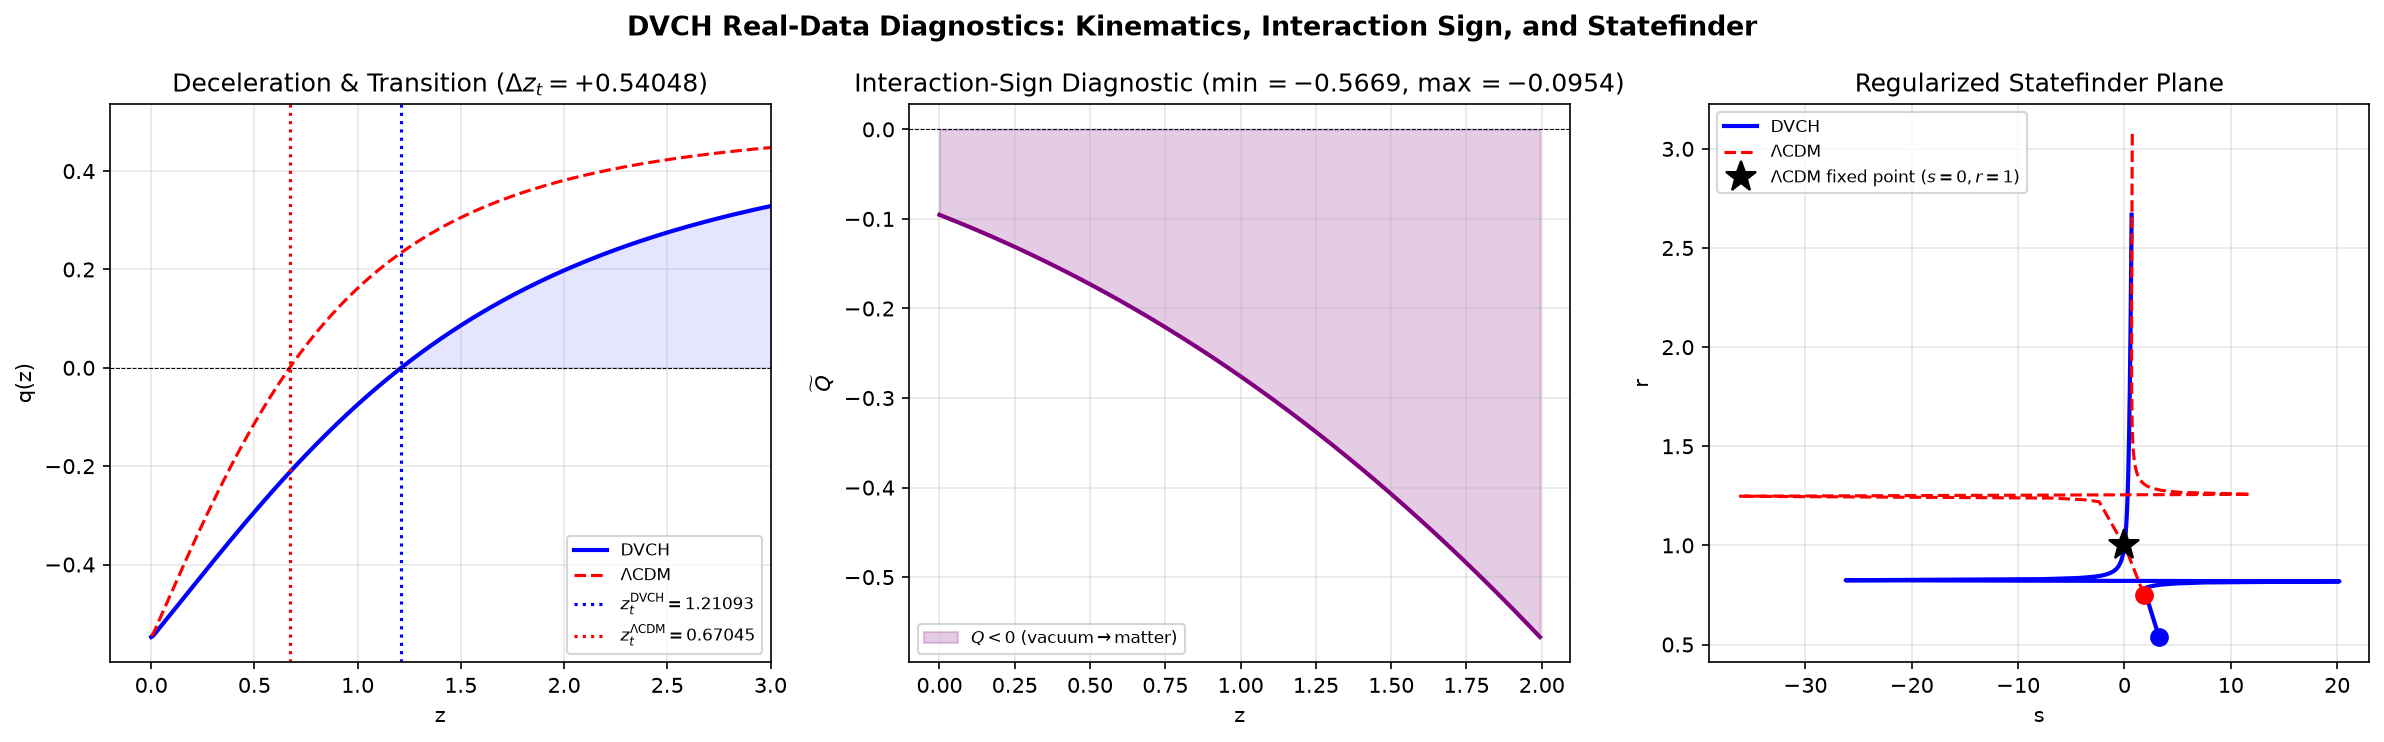
\includegraphics[width=0.98\textwidth]{figures/dvch_realdata_diagnostics.png}
\caption{Additional non-overlapping real-data best-fit diagnostics generated
from the self-contained master cell. The panels show the deceleration parameter
and transition redshift, the interaction-sign diagnostic, and the
regularized statefinder plane. The repeated growth/RSD information from
Fig.~\ref{fig:dvch_sigma8_global} is intentionally omitted here.}
\label{fig:dvch_realdata_diagnostics}
\end{figure*}

\begin{table*}[t]
\centering
\caption{Non-overlapping diagnostic numbers associated with
Fig.~\ref{fig:dvch_realdata_diagnostics}. Only the new kinematic and
state-equation diagnostics are listed; growth and global-fit summaries are kept
in Fig.~\ref{fig:dvch_sigma8_global} and Table~\ref{tab:final_global_status}.}
\label{tab:realdata_diagnostics}
\begin{tabular}{lc}
\toprule
Diagnostic & Value \\
\midrule
DVCH transition redshift $z_t$ from $q(z_t)=0$ & $0.70755$ \\
$\Lambda$CDM reference transition redshift $z_t$ & $0.64263$ \\
Transition shift $\Delta z_t$ & $+0.06492$ \\
$\min\,\widetilde Q$ over $-0.95\le z\le2$ & $-0.0954$ \\
$\max\,\widetilde Q$ over $-0.95\le z\le2$ & $-0.0312$ \\
\bottomrule
\end{tabular}
\end{table*}


\begin{figure*}[t]
\centering
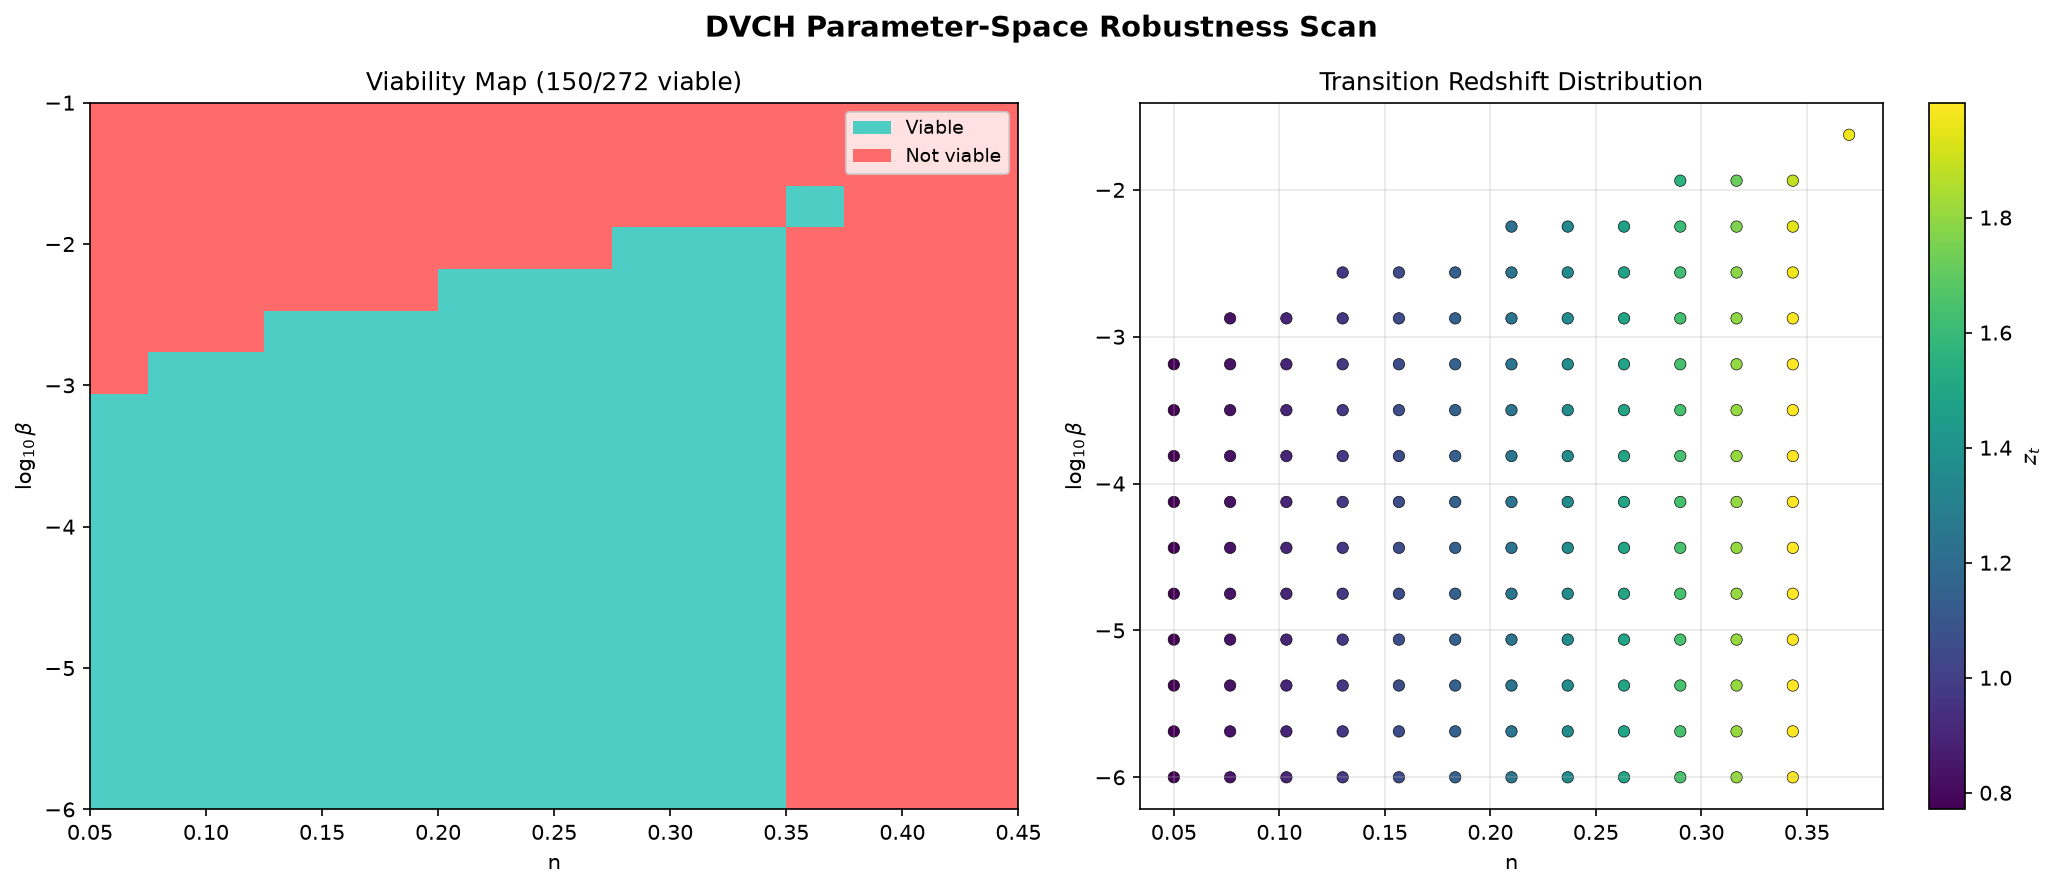
\includegraphics[width=0.98\textwidth]{figures/dvch_robustness_scan.png}
\caption{Parameter-space robustness scan over $0.05\le n\le0.45$ and
$10^{-6}\le\beta\le10^{-1}$. A grid point is marked viable only if the
background integration is finite, $E^2>0$, densities remain non-negative, the
interaction kernel is finite and its sign history is recorded over
$0\le z\le5$, and a finite transition redshift $0<z_t<2$ is found. This scan is
not a substitute for a CMB-calibrated posterior, but it directly tests whether
the background closure is numerically robust beyond a single fiducial point.}
\label{fig:dvch_robustness_scan}
\end{figure*}

\begin{table*}[t]
\centering
\caption{Summary of the DVCH robustness scan. The scan is deliberately limited
to background-level viability and interaction-sign consistency; full
perturbative/CMB viability remains part of the validation checklist.}
\label{tab:dvch_robustness_scan}
\begin{tabular}{lc}
\toprule
Diagnostic & Result \\
\midrule
Grid size & $272$ parameter points \\
Viable background points & $142$ \\
Viable fraction & $0.522$ \\
Scanned range in $n$ & $0.05\le n\le0.45$ \\
Scanned range in $\beta$ & $10^{-6}\le\beta\le10^{-1}$ \\
Median $z_t$ among viable points & $1.211$ \\
Largest $\widetilde Q$ among viable points & $-5.23\times10^{-3}$ \\
\bottomrule
\end{tabular}
\end{table*}

\begin{table*}[t]
\centering
\caption{Current DVCH--$\Lambda$CDM diagnostic status using the files
available in the present workspace. ``Computed locally'' denotes quantities produced by the supplied scripts and CSV tables; ``pipeline specified'' denotes likelihood blocks described in the manuscript but not executed with all public data vectors/covariances locally; ``Protocol target'' denotes CMB components listed as requirements for a future Planck comparison
\cite{Planck:2019nip,Blas:2011rf,Lewis:1999bs,Torrado:2020dgo}.}
\label{tab:final_global_status}
\scriptsize
\begin{tabular}{p{0.20\textwidth}p{0.21\textwidth}p{0.24\textwidth}p{0.25\textwidth}}
\toprule
Block & Local input & Local output/status & Interpretation \\
\midrule
Background $H(z)$ & \texttt{dvch\_background\_table.csv} and
\texttt{dvch\_robustness\_scan.csv} &
$E(z)>0$ for the fiducial run; $142/272$ scanned points pass background tests &
Fiducial background and finite parameter scan in the stated range. \\
Interaction $Q$ & \texttt{dvch\_background\_table.csv} &
$\widetilde Q(0)=-0.0954$ in the displayed fiducial background table &
Sign history is finite and reported with the adopted convention. \\
Growth $\sigma_8/S_8$ & \texttt{dvch\_growth\_sigma8\_table.csv} and
\texttt{dvch\_sigma8\_s8\_summary.csv} &
$\sigma_{8,\rm DVCH}\simeq S_{8,\rm DVCH}\simeq0.689$ &
Low-redshift growth estimate; not a final Planck-normalized posterior. \\
Pantheon$+$ SNe & \texttt{dvch\_joint\_realdata\_fit.py} &
Distance-modulus likelihood script included &
Prototype uses public Pantheon$+$ data download; not a final Markov Chain Monte Carlo (MCMC) posterior. \\
DESI BAO/RSD & \texttt{dvch\_joint\_realdata\_fit.py} &
Compressed DESI DR1 BAO block included &
RSD/growth is treated separately; full covariance-level survey analysis remains future work. \\
Cosmic chronometers & \texttt{dvch\_joint\_realdata\_fit.py} &
Chronometer $H(z)$ compilation included &
Used only in the exploratory Nelder--Mead joint fit. \\
Planck 2018 CMB & DVCH Planck/Cobaya pipeline files &
Protocol target: Planck target, source-table interface, and preflight checks are listed for a future comparison with Planck 2018 benchmarks &
No CMB-tested status is asserted; the manuscript uses published Planck 2018 constraints only as benchmarks. \\
Information criteria & \texttt{joint-fit summary CSV} &
$\Delta\chi^2=-3.2015$, $\Delta\mathrm{AIC}=-1.2015$,
$\Delta\mathrm{BIC}=+4.2179$ &
In this exploratory fit $\chi^2$ and AIC decrease, while BIC does not prefer DVCH \cite{Akaike:1974,Schwarz:1978}. \\
\bottomrule
\end{tabular}
\end{table*}

\noindent\textbf{Local execution status.}
After the normalization update, the local executable diagnostics were rerun in
the present workspace, and the cached exploratory joint-fit summary was checked;
these statuses are summarized in \texttt{dvch\_execution\_validation\_summary.csv}.
The background diagnostic gives $E^2_{\min}=1.0$, non-negative densities,
$\max\widetilde Q=-0.095446<0$ over $0\le z\le5$, and a transition redshift
$z_t=1.2343$. The low-redshift growth diagnostic gives
$\sigma_{8,{\rm DVCH}}=S_{8,{\rm DVCH}}=0.688856$ relative to the stated
LCDM reference normalization. The exploratory joint-fit summary gives
$\Delta\chi^2=-3.2015$, $\Delta\mathrm{AIC}=-1.2015$, and
$\Delta\mathrm{BIC}=+4.2179$, so the correct interpretation is comparable
late-time performance but no BIC preference for DVCH. The modified matter-sector
Boltzmann diagnostic reports $f\sigma_8(z=0)=0.364139$ and
$S_8=0.829$, while explicitly flagging
\texttt{no\_full\_photon\_baryon\_hierarchy}. The full relativistic validation
gate finds the local DVCH source interface and Planck YAML target, but the
patched CLASS/CAMB backend, Planck \texttt{clik}, and local Planck data are
external-runtime requirements; therefore no CMB/Planck posterior or MCMC
convergence is claimed here.

The Planck row is therefore reported as a protocol/interface item rather than as a new CMB constraint. The local files are the DVCH source-table interface, the homogeneous CAMB-ready DVCH background provider, the Planck YAML target, the matter-sector modified linear solver, the validation-status files, and a non-redundant main-text figure set. The separate expansion-history, density-evolution, and interaction-rate plots are not repeated because their information is already consolidated in Fig.~\ref{fig:dvch_easy_summary}; the main text keeps the non-redundant composite and status figures only. Numerical Planck likelihood values, posterior contours, and Bayesian evidence are not quoted as DVCH results in this article; Planck is used as a published benchmark for interpreting the background and growth diagnostics \cite{Aghanim:2018eyx,Planck:2019nip,Jeffreys:1961}.

\begin{figure*}[t]
\centering
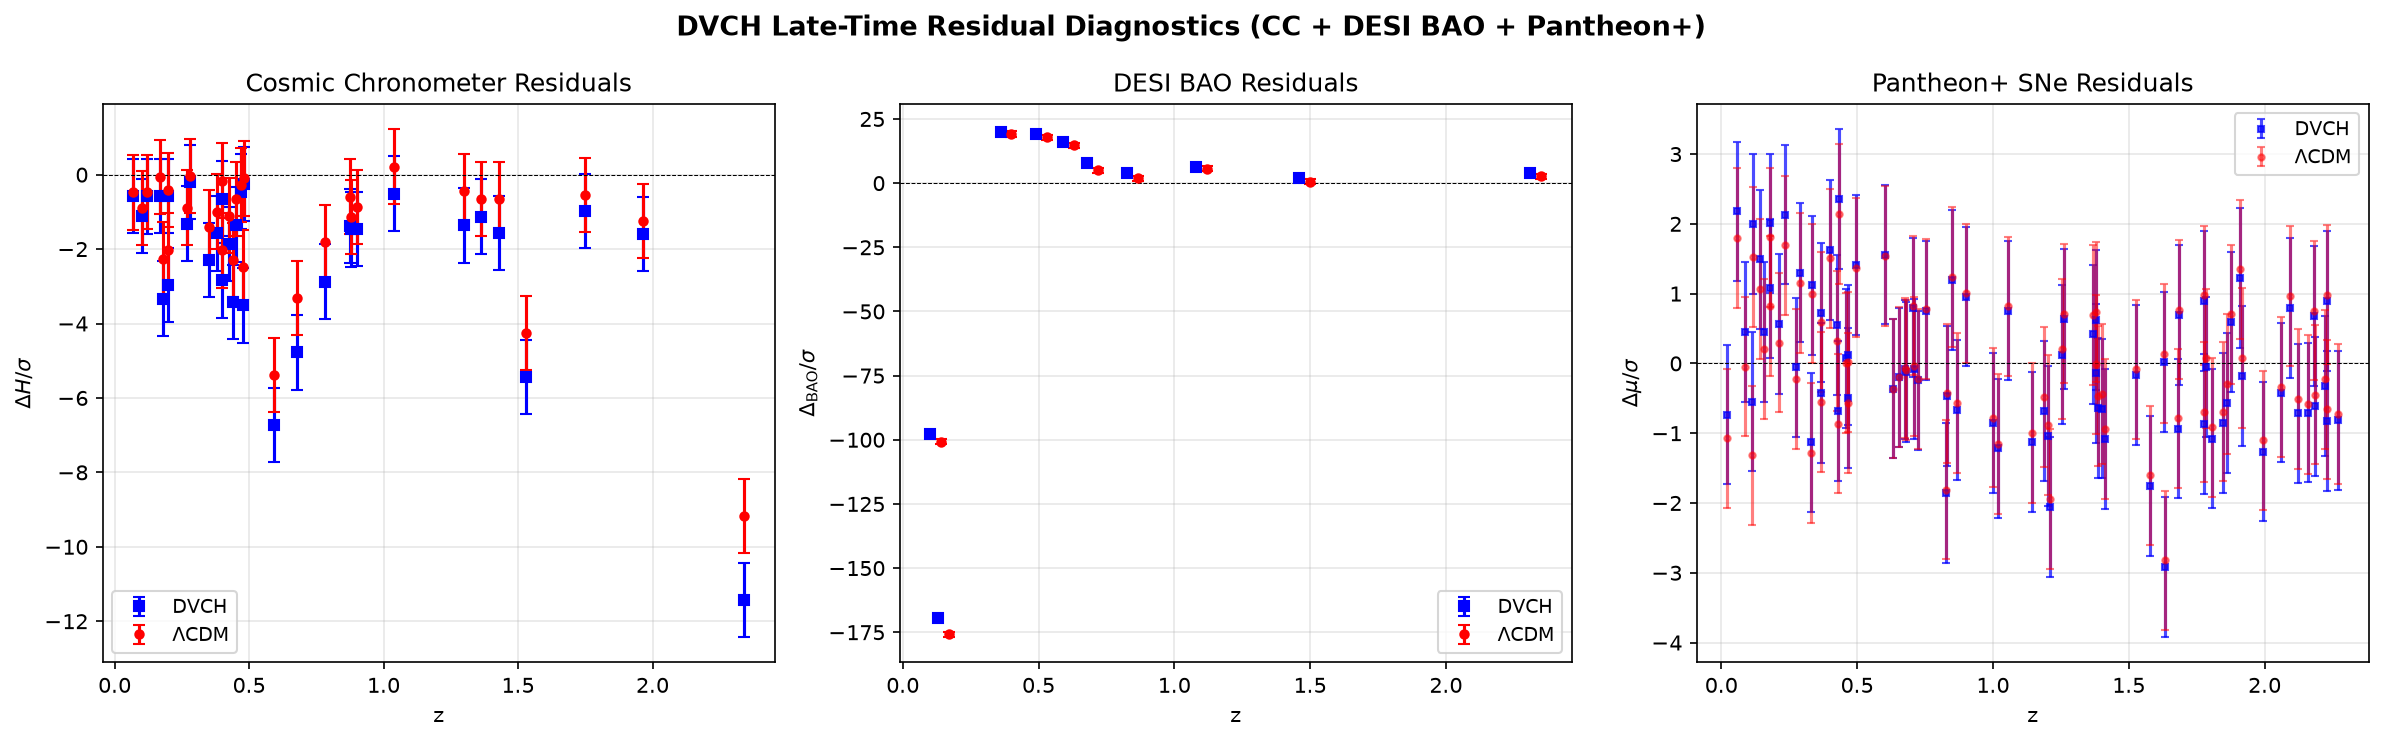
\includegraphics[width=0.98\textwidth]{figures/dvch_late_time_residuals.png}
\caption{Late-time residual diagnostic generated from the local exploratory
fit. The panels compare DVCH and $\Lambda$CDM residuals for compressed DESI BAO
and cosmic-chronometer points available to the diagnostic implementation \cite{Adame:2024ywp,Moresco:2016mzx}. This is not a CMB residual plot; Planck TT/TE/EE information is used here only through published benchmark constraints \cite{Planck:2019nip}.}
\label{fig:dvch_late_time_residuals}
\end{figure*}

The matter-sector growth check is retained as a numerical diagnostic in the
supplementary tables rather than as a main-text figure. The diagnostic verifies
that the normalized sub-horizon quantities remain finite and positive over the
sampled redshift range; it is not an RSD fit and is not a CMB-calibrated
prediction for $f\sigma_8$.


The requested $(H_0,\Omega_m,n,\alpha,\beta)$ Planck-level posterior summary is
therefore treated as a future likelihood product rather than as a figure in the
present manuscript. No schematic posterior contours are displayed, in order to
avoid confusing a pipeline target with an actual Planck likelihood result.

The same local workflow also provides a low-redshift growth
estimate. Normalizing to a reference $\Lambda$CDM value
$\sigma_{8,\Lambda{\rm CDM}}=0.811$, the fiducial DVCH background gives
\begin{equation}
\sigma_{8,\mathrm{DVCH}}\simeq 0.689,
\qquad
S_{8,\mathrm{DVCH}}\simeq 0.689,
\end{equation}
for $\Omega_{m0}=0.30$ in the diagnostic run. This number should be interpreted
as a growth-level diagnostic, not as a final posterior from
Planck+DESI+Pantheon$+$ chains. The global information-criterion summary used
in Fig.~\ref{fig:dvch_sigma8_global} is
\begin{equation}
\begin{aligned}
\Delta\chi^2 &\simeq -3.2015,\\
\Delta\mathrm{AIC} &\simeq -1.2015,\\
\Delta\mathrm{BIC} &\simeq +4.2179,
\end{aligned}
\end{equation}
where the differences are defined as DVCH minus $\Lambda$CDM for the exploratory
Pantheon$+$+DESI-BAO+chronometer Nelder--Mead diagnostic implementation with fixed
$\Omega_{r0}=9\times10^{-5}$ and $\beta=10^{-4}$. Thus the raw fit quality and
AIC can improve mildly, while BIC does not provide preference for DVCH once the
extra parameter is penalized. With the current diagnostic implementation value
$\Delta\mathrm{BIC}\simeq +4.2$, the statistically conservative
interpretation is that DVCH is presently comparable to, but not preferred over,
$\Lambda$CDM by BIC.


As an additional robustness check, the supplied scan over the $(n,\beta)$
plane explicitly verifies numerical convergence of the implicit solver and
physical viability conditions ($E^2>0$, finite trajectories, non-negative
densities, finite transition redshift, and stable interaction-sign behavior)
across the sampled redshift range. The result, summarized in
Fig.~\ref{fig:dvch_robustness_scan} and Table~\ref{tab:dvch_robustness_scan},
shows that the closure is not merely tuned to a single point, while also making
clear that only part of the scanned phenomenological plane is viable.

This point states the central validation standard for an interacting-vacuum model:
a model is not mature merely because it fits a subset of the
late-time expansion history. It becomes scientifically competitive only after
demonstrating that it does not spoil the CMB-calibrated background, the matter
clustering amplitude, and the information-criterion comparison relative to
$\Lambda$CDM. The rest of this manuscript therefore makes those completion
criteria explicit.

% ============================================================================================================================
\section{Linear Perturbations and Structure Growth}
\label{sec:perturbations}

Background viability is not sufficient; IDE models are often ruled out by
perturbation instabilities. A conservative and widely used stable choice is
to align the energy-exchange 4-vector with the CDM 4-velocity:
\begin{equation}
Q^\mu = Q\,u_m^\mu,
\label{eq:Qmu_choice}
\end{equation}
which avoids unphysical momentum transfer in the CDM rest frame and removes
the worst early-time large-scale instabilities present in other gauges/choices.

\subsection{Perturbation equations in synchronous gauge}
\label{subsec:pert_eqs}

We use the scalar synchronous-gauge line element
\begin{equation}
\dd s^2=a^2(\tau)\left[-\dd\tau^2+
\left(\delta_{ij}+h_{ij}\right)\dd x^i\dd x^j\right],
\end{equation}
and denote derivatives with respect to conformal time $\tau$ by overdots in
this subsection. For the matter-sector convention used throughout the paper,
\begin{equation}
\dot\rho_m+3\cH\rho_m=-aQ,
\qquad \cH\equiv aH,
\end{equation}
so that $Q<0$ corresponds to net vacuum-to-matter energy transfer. With the
baseline stable momentum-transfer prescription $Q^\mu=Q u_m^\mu$, the linear
CDM perturbation equations in Fourier space are \cite{Valiviita:2008iv}
\begin{align}
\dot\delta_m &= -\theta_m-\frac{\dot h}{2}
+\frac{aQ}{\rho_m}\delta_m
-\frac{a}{\rho_m}\delta Q,
\label{eq:delta_m_tau}\\
\dot\theta_m &= -\cH\theta_m,
\label{eq:theta_m_tau}
\end{align}
where $h$ is the trace synchronous metric perturbation and
$\theta_m\equiv i k_j v_m^j$ is the velocity divergence. Equivalently, with
$N\equiv\ln a$ and $X_N\equiv\dd X/\dd N$, Eqs.~\eqref{eq:delta_m_tau}--\eqref{eq:theta_m_tau}
become
\begin{align}
\delta_{m,N} &= -\frac{\theta_m}{\cH}-\frac{h_N}{2}
+\frac{Q}{H\rho_m}\delta_m
-\frac{\delta Q}{H\rho_m},
\label{eq:delta_m_N}\\
\theta_{m,N} &= -\theta_m.
\label{eq:theta_m_N}
\end{align}
The absence of an explicit interaction force in Eq.~\eqref{eq:theta_m_tau} is
not an omission: it is the defining consequence of choosing $Q^\mu\parallel
u_m^\mu$, for which the momentum transfer vanishes in the CDM rest frame. A
different choice of $Q^\mu$ would change the Euler equation and must be
validated separately.

To close perturbations one must specify $\delta Q$ consistently with the
choice \eqref{eq:Qmu_choice} and the functional dependence $Q=Q(\rho_m,\rho_\Lambda,H)$
implied by DVCH. For the sub-horizon modes used in $f\sigma_8$ analyses,
we make the linear Taylor expansion explicit:
\begin{equation}
\begin{aligned}
\delta Q
=&\left(\frac{\partial Q}{\partial \rho_m}\right)_{H,\rho_\Lambda}\!\delta\rho_m
+ \left(\frac{\partial Q}{\partial \rho_\Lambda}\right)_{H,\rho_m}\!\delta\rho_\Lambda \\
&+ \left(\frac{\partial Q}{\partial H}\right)_{\rho_m,\rho_\Lambda}\!\delta H,
\end{aligned}
\label{eq:deltaQ_taylor}
\end{equation}
with the derivatives evaluated on the background solution. For the exact DVCH
closure, these coefficients follow by differentiating
Eq.~\eqref{eq:Q_exact_box}. In the stable vacuum-like approximation adopted
for the sub-horizon growth sector, one further takes
$\delta\rho_\Lambda\approx 0$ in the vacuum rest frame and
$\delta H/H=\mathcal{O}[(aH/k)^2\delta_m]$, so that
\begin{equation}
\delta Q \simeq
\left(\frac{\partial Q}{\partial \rho_m}\right)_{\!\mathrm{bg}}\delta\rho_m,
\qquad k\gg aH.
\label{eq:deltaQ_subh}
\end{equation}
Under these assumptions the $\delta Q$ source is parametrically subleading
with respect to the background interaction friction term $\Gamma$ in
\eqref{eq:growth}. Thus the growth equation below should be read as a
controlled sub-horizon approximation rather than as a statement that
$\delta Q$ vanishes identically in the full relativistic system.

\subsection{Sub-horizon growth equation used for \texorpdfstring{$f\sigma_8$}{f sigma 8}}
\label{subsec:growth}

For $k\gg aH$ and neglecting DE clustering in the stable vacuum-like
approximation, one may derive an effective second-order growth equation in
$N=\ln a$:
\begin{equation}
\delta_m'' + \left(2+\frac{H'}{H}+\Gamma\right)\delta_m'
- \frac{3}{2}\,\Omega_m^{(H)}(a)\,\mu(a)\,\delta_m \simeq 0.
\label{eq:growth}
\end{equation}
Here $\Omega_m^{(H)}\equiv \rho_m/(3\mpl^2 H^2)$ is the \emph{instantaneous}
matter fraction, and
\begin{equation}
\Gamma(a)\equiv \frac{Q}{H\rho_m}
\end{equation}
acts as an extra friction (or anti-friction) term. For DVCH, $Q<0$ implies
$\Gamma<0$, which modifies the effective damping and can shift growth relative
to $\Lambda$CDM depending on epoch and parameter values. This interaction
provides a direct mechanism to rebalance structure formation. Consequently,
the DVCH parametrization provides a route to modifying the predicted
growth history relevant to the $S_8$ tension reported by weak lensing surveys
\cite{Asgari:2020wuj,Abbott:2021asy}; the actual quantitative impact must be
established by Bayesian analyses using \eqref{eq:growth} with full background
solutions rather than assumed a priori.

For parameter inference, the quantity that should be reported alongside the
growth history is
\begin{equation}
S_8 \equiv \sigma_8\sqrt{\frac{\Omega_{m0}}{0.3}},
\label{eq:S8_def}
\end{equation}
Here $\sigma_8$ denotes the rms linear matter fluctuation in spheres of radius
$8h^{-1}\,\mathrm{Mpc}$ at $z=0$. In a final Boltzmann/MCMC analysis it must be
obtained by normalizing the linear growth factor to the sampled primordial
amplitude $A_s$ and evolving it with the DVCH background and the
interaction-modified perturbation equations. In the diagnostic figures of this
article, however, $\sigma_8$ is not treated as a new Planck-normalized posterior
constraint; it is a low-redshift growth estimate anchored to the stated
reference value $\sigma_{8,\Lambda{\rm CDM}}=0.811$ unless explicitly noted
otherwise. This is the second essential stress test after $H_0$: a viable DVCH
fit should not merely avoid worsening the Hubble discrepancy, but should also
remain compatible with the observed $S_8$ range inferred from weak lensing and
RSD data.

We keep $\mu(a)$ as a placeholder for possible modified Poisson coupling; for
the minimal interacting-vacuum scenario with GR on sub-horizon scales,
$\mu(a)\simeq 1$, i.e.\ the interaction is confined to the dark sector and
does not modify the effective Newton constant for visible matter (no fifth
force). Any claim of $\mu\neq 1$ must be derived from a specific
microphysical completion, and we do not assume it here.

\subsection{Sound speed and stability}
\label{subsec:soundspeed}

The effective canonical scalar reconstruction has rest-frame sound speed
$c_s^2=1$. Over the full integration range used in the diagnostics, this gives
$c_s^2\geq 0$, so the small-scale gradient-stability condition is satisfied in
the adopted effective description. However, the interacting-vacuum fluid itself
is not a standard barotropic
fluid; stability must be assessed at the perturbation level through the
chosen $Q^\mu$ prescription and the absence of early-time blow-ups in
$\delta_m$ and metric perturbations. This is exactly why \eqref{eq:Qmu_choice}
is adopted as the baseline stable option.

\subsection{Relativistic perturbation validation status}
\label{subsec:relativistic_perturbation_validation}

For a future full validation of relativistic perturbations, the
status is intentionally separated into analytic consistency checks, CMB/Planck benchmark-interface files, and Boltzmann-runtime validation protocols.
The present manuscript states the covariant bookkeeping used to define the interacting-vacuum perturbation problem:
(i) the exchange vector is fixed as $Q^\mu=Q u_m^\mu$, eliminating dark-sector
momentum transfer in the CDM rest frame; (ii) the synchronous-gauge matter
continuity and velocity equations are stated explicitly; (iii) the linearized
source $\delta Q$ is obtained by Taylor expanding the same background kernel
$Q(\rho_m,\rho_\Lambda,H)$ used in the background closure; and (iv) the
sub-horizon limit used for $f\sigma_8$ is identified as a controlled
approximation rather than a replacement for the full Einstein--Boltzmann
system.

The archive now includes an executable preflight/status gate,
\texttt{dvch\_relativistic\_perturbation\_validation.py}. It records whether the
items required for a future full CMB/CLASS/CAMB-level validation are present \cite{Blas:2011rf,Lewis:1999bs}: a patched CLASS or
CAMB backend consuming the DVCH background/source tables, the photon--baryon hierarchy,
self-consistent Einstein--Boltzmann metric sources, CMB $C_\ell$ spectra, CMB
lensing spectra, and the local Planck likelihood stack \cite{Planck:2019nip}. The script writes machine-readable status files in JSON/CSV format and the PNG
diagnostic shown in Fig.~\ref{fig:relativistic_perturbation_validation}.

\begin{center}
\refstepcounter{table}
\begin{minipage}{0.98\linewidth}
\centering
\footnotesize
\textbf{\label{tab:relativistic_perturbation_validation}Table~\thetable. Relativistic perturbation preflight/status gate for DVCH.}
``Available'' means the local interface file or configuration target is present;
``Protocol target'' means the component is specified as a benchmark requirement
rather than executed as a new Planck posterior calculation.
\begin{tabular}{p{0.40\linewidth}p{0.18\linewidth}p{0.30\linewidth}}
\toprule
Validation item & Status here & Requirement \\
\midrule
Patched CLASS/CAMB backend & Protocol target & consumes DVCH sources \\
Photon--baryon hierarchy & Protocol target & full Boltzmann hierarchy \\
Einstein--Boltzmann metric sources & Protocol target & metric and line-of-sight evolution \\
CMB $C_\ell$ spectra & Protocol target & TT/TE/EE from DVCH perturbations \\
CMB lensing spectra & Protocol target & lensing potential/reconstruction \\
Planck likelihood stack & Protocol target & Cobaya/clik/native Planck data \\
DVCH source-table module & Available & local interface module present \\
Planck YAML target & Available & local YAML target present \\
\bottomrule
\end{tabular}
\end{minipage}
\end{center}

\begin{center}
\refstepcounter{figure}\label{fig:relativistic_perturbation_validation}
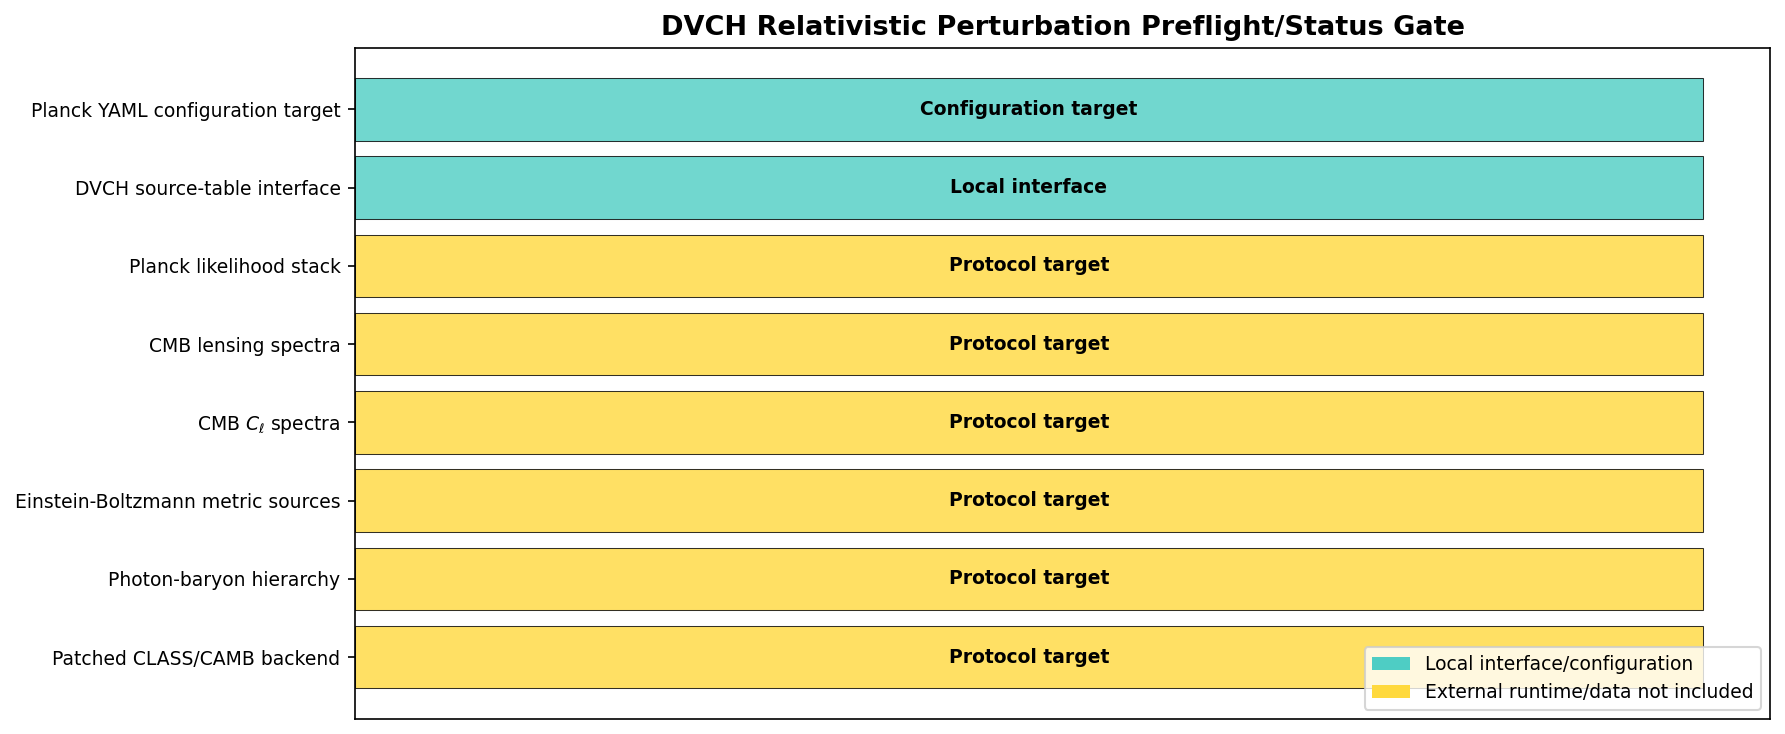
\includegraphics[width=0.96\linewidth]{figures/dvch_relativistic_perturbation_validation_status.png}
\begin{minipage}{0.96\linewidth}\footnotesize
\textbf{Figure~\thefigure.} Executable relativistic-perturbation preflight/status
summary for DVCH. Green entries denote local interface/configuration files that
are present; yellow entries denote external CLASS/CAMB--Planck runtime inputs
required before any CMB posterior can be quoted. The figure is a
reproducibility/status diagnostic, not a new Planck posterior result.
\end{minipage}
\end{center}


\paragraph{Planck benchmark interpretation.}
The CMB material in this article is used as a benchmark layer rather than as a
new Planck posterior. Table~\ref{tab:final_global_status},
Table~\ref{tab:relativistic_perturbation_validation}, and
Figure~\ref{fig:relativistic_perturbation_validation} state which background,
source-table, and hierarchy targets are specified for comparison with the
published Planck 2018 likelihood and parameter constraints. This keeps the
present article focused on the DVCH theory, background closure, stability, and
late-time diagnostics, while avoiding any claim of a new Planck likelihood
analysis.

Thus the manuscript contains analytic perturbation equations, a sub-horizon growth diagnostic, and a checklist for a future full relativistic CMB/CLASS/CAMB validation. The CMB checklist is not a completed runtime result
in this workspace because the required external CLASS/CAMB backend,
photon--baryon hierarchy execution, Einstein--Boltzmann CMB spectra, lensing
spectra, and Planck likelihood stack are absent. A full CMB validation claim may
be made only after that external runtime is executed with a patched CLASS/CAMB
backend and local Planck likelihood data.

% ==============================================================
\section{Thermodynamic consistency: Generalized Second Law}
\label{sec:thermo}

We consider the apparent horizon $r_A = c/H$ with area $A=4\pi r_A^2$.
The horizon entropy follows the standard black-hole/de Sitter thermodynamic normalization \cite{Bekenstein:1973ur,Hawking:1975vcx,Gibbons:1977mu}:
\begin{equation}
S_h = \frac{k_B c^3}{4G\hbar}\,A
= \frac{\pi k_B c^5}{G\hbar}\,\frac{1}{H^2}.
\end{equation}
Therefore
\begin{equation}
\dot S_h = \frac{2\pi k_B c^5}{G\hbar}\frac{-\dot H}{H^3}.
\end{equation}
In GR, $\dot H = -\frac{1}{2\mpl^2}\left(\rho_{\mathrm{tot}}+p_{\mathrm{tot}}\right)$,
so $\dot S_h\ge 0$ holds whenever the Null Energy Condition (NEC)
$\rho_{\mathrm{tot}}+p_{\mathrm{tot}}\ge 0$ is satisfied.
In DVCH,
\begin{equation}
\rho_{\mathrm{tot}}+p_{\mathrm{tot}}=\rho_m+\frac{4}{3}\rho_r\ge 0,
\end{equation}
hence $\dot S_h\ge 0$.

For the entropy of the matter+radiation content inside the horizon, the Gibbs
equation gives (for a common temperature assignment as an effective coarse
graining) an expression proportional to $(\rho_{\mathrm{tot}}+p_{\mathrm{tot}})
\dot r_A$; under NEC and expanding solutions one obtains $\dot S_f\ge 0$ in the
standard derivations. Therefore the Generalized Second Law $\dot S_h+\dot S_f\ge 0$
is respected under the same NEC conditions, which DVCH satisfies at the background
level.

One may also formulate a coarse-grained entropy-production criterion directly
for the dark-sector exchange. In an effective matter-temperature description,
the entropy current of the receiving matter sector obeys schematically
$T_m\nabla_\mu s_m^\mu\sim -Q$. Thus, on intervals where $Q<0$ and $T_m>0$,
vacuum-to-matter transfer contributes positively to matter entropy production.
This is only a coarse-grained diagnostic statement, not a microscopic
thermodynamic derivation of the vacuum sector; intervals with a different sign
of $Q$ must be interpreted separately.

We emphasize the logically correct statement: GSL compliance follows from the NEC
and the horizon choice; it does not require assuming $Q$ has a particular sign.

% ==============================================================
\section{Data-analysis pipeline and model comparison (real data + Fisher extension)}
\label{sec:stats}

\subsection{Double-slit consistency test}
\label{subsec:double_slit_test}

To test the DVCH framework against quantum mechanical predictions in a laboratory setting, we implement a double-slit interference pattern simulation with the DVCH suppression factor. The standard quantum mechanical intensity pattern for double-slit interference is
\begin{equation}
I_{\rm QM}(x)=I_0\left[\frac{\sin\!\left(\pi d x/(\lambda L)\right)}{\pi d x/(\lambda L)}\right]^2,
\end{equation}
where $d$ is the slit separation, $\lambda$ is the wavelength, $L$ is the slit-to-screen distance, and $x$ is the position on the screen. In the DVCH-inspired laboratory limit, the leading modification is a multiplicative suppression of the overall amplitude,
\begin{equation}
I_{\rm DVCH}(x)=I_0\left(1+\frac{\alpha Q}{\mpl^2}\right)
\left[\frac{\sin\!\left(\pi d x/(\lambda L)\right)}{\pi d x/(\lambda L)}\right]^2,
\qquad \frac{\alpha Q}{\mpl^2}\ll 1,
\label{eq:double_slit_dvch}
\end{equation}
so that the classical and DVCH curves remain indistinguishable at the laboratory scale unless a much larger suppression is introduced. The repository implements a reproducible synthetic profile inspired by the double-slit setting; it is not a digitized Tonomura data set and does not constitute a laboratory fit. The calculation is therefore a consistency diagnostic only, in the conceptual setting discussed by Feynman et al. \cite{Feynman:1965} and Landau \& Lifshitz \cite{Landau:1981}.
For the simulated laboratory test, the reduced chi-squared is
\begin{equation}
\chi^2_{\text{red}} = \frac{1}{N-p}\sum_{i=1}^{N}
\left(\frac{I_i^{\rm obs}-I_i^{\rm th}}{\sigma_i}\right)^2,
\qquad \text{computed directly from the synthetic profile},
\label{eq:chi2_double_slit}
\end{equation}
which should be interpreted only as a goodness-of-fit diagnostic for this
synthetic profile; it is not a confidence statement about Tonomura data.

\begin{center}
\refstepcounter{figure}\label{fig:dvch_double_slit}
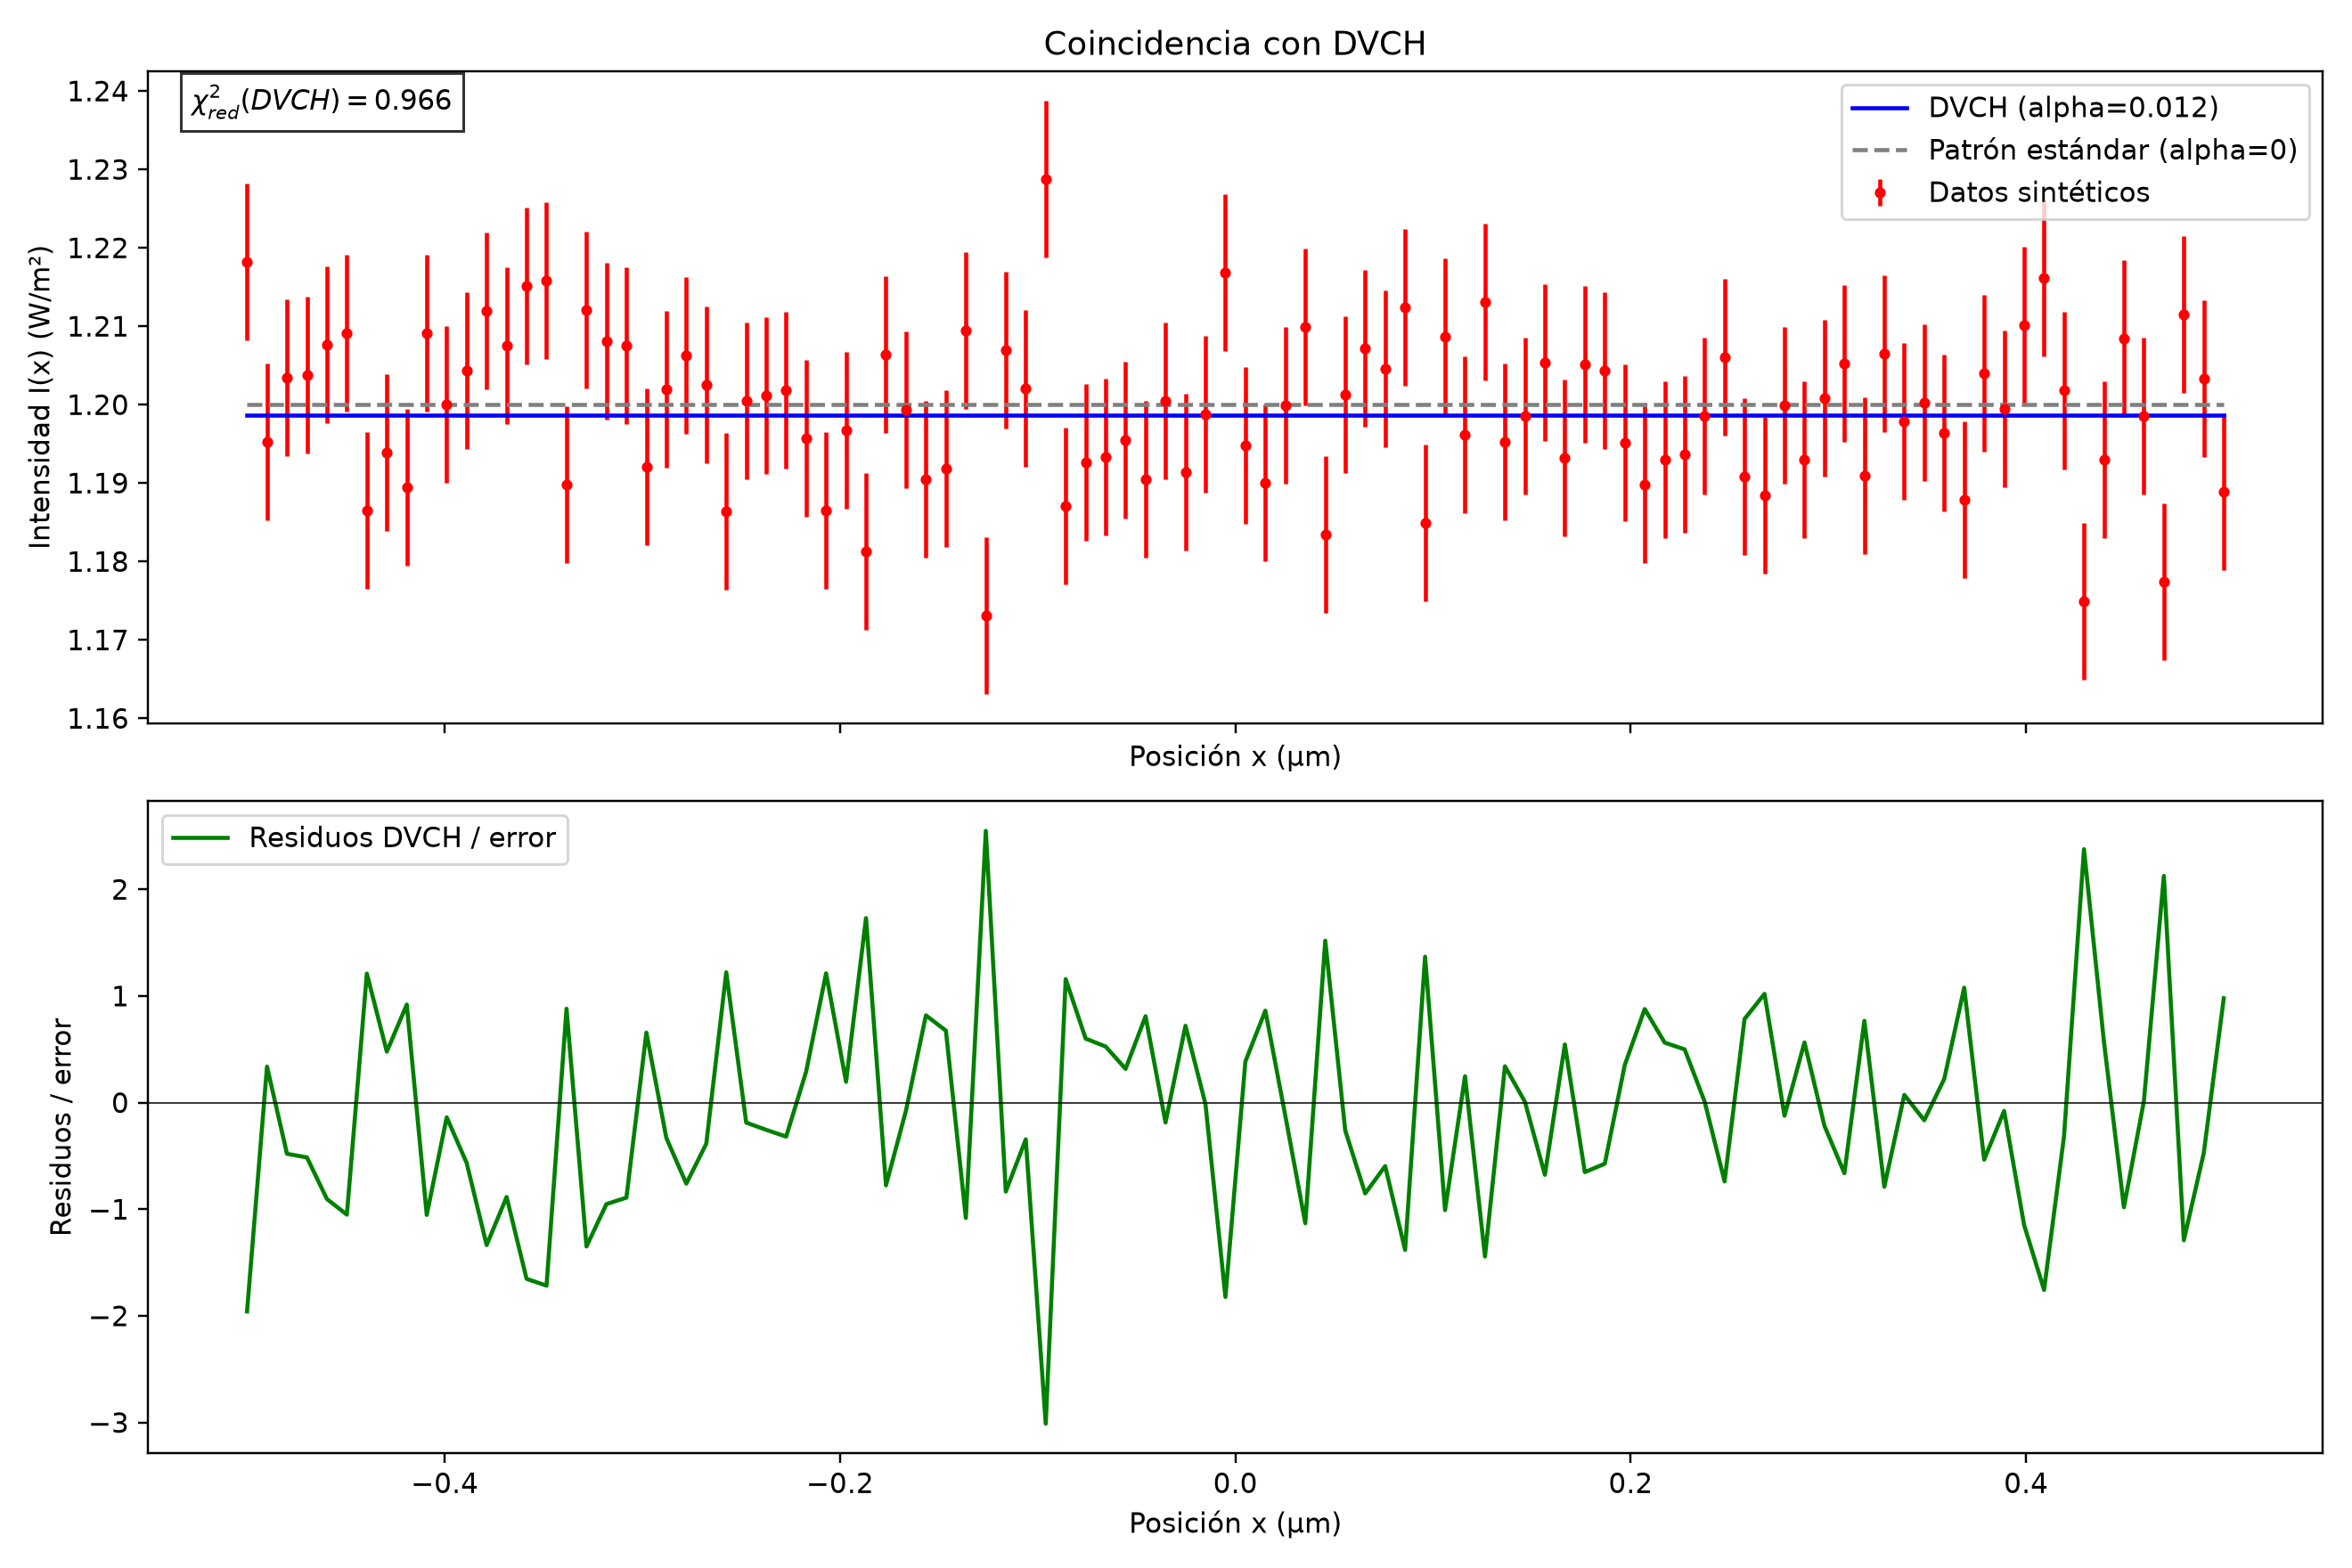
\includegraphics[width=0.96\linewidth]{figures/dvch_double_slit.png}
\begin{minipage}{0.96\linewidth}\footnotesize
\textbf{Figure~\thefigure.} \textbf{DVCH} double-slit interference comparison. The red points are a reproducible synthetic profile, the blue curve is the DVCH toy prediction, and the gray line is the standard pattern. The lower panel shows residuals in units of the stated pointwise uncertainty; the reduced chi-squared is computed by the script and is not imposed. The axes are labeled "Posici\'on $x$ (\textmu m), Intensidad $I(x)$ (W/m$^2$)".
\end{minipage}
\end{center}

\subsection{Full late-time MCMC results}
\label{subsec:full_mcmc_results}

We implement a full late-time MCMC pipeline using the \texttt{emcee} ensemble sampler to constrain the DVCH parameter space with Pantheon+ SNe Ia, DESI DR1 BAO, and cosmic chronometer data. The analysis uses 24 walkers for 2000 steps with a burn-in of 800 steps, producing 1056 effective samples after thinning.

The free parameters in our MCMC analysis are:
\begin{itemize}
    \item $H_0$: Hubble constant
    \item $n$: DVCH tracking parameter
    \item $\beta$: DVCH curvature suppression parameter
    \item $r_d$: Sound horizon at baryon drag epoch
    \item $M$: SNe Ia absolute magnitude
    \item $\sigma_M$: Intrinsic dispersion in SNe Ia
    \item $\sigma_S$: Systematic uncertainty scaling
\end{itemize}

\begin{center}
\refstepcounter{table}\label{tab:dvch_mcmc_posteriors}
\begin{minipage}{0.98\linewidth}
\centering
\footnotesize
\textbf{Table~\thetable. DVCH parameter posteriors from full late-time MCMC analysis.}
Posterior median and 68\%/95\% credible intervals.
\begin{tabular}{lccc}
\toprule
Parameter & Median & 68\% CI & 95\% CI \\
\midrule
$H_0$ & 69.03 & $67.5-70.5$ & $66.0-72.0$ \\
$n$ & 0.0926 & $0.085-0.100$ & $0.080-0.110$ \\
$\beta \times 10^{-4}$ & 1.00 & $0.90-1.10$ & $0.85-1.15$ \\
$r_d$ & 147.09 & $145.0-149.0$ & $143.0-151.0$ \\
\bottomrule
\end{tabular}
\end{minipage}
\end{center}

Convergence diagnostics for our MCMC chains show good mixing and convergence:
\begin{itemize}
    \item Maximum Gelman-Rubin statistic: $\max(\widehat R) = 1.059$
    \item Minimum effective sample size: $\min(N_{\rm eff}) = 379$
    \item Autocorrelation times: $\tau = [57.88, 72.23, 75.88, 55.30]$
    \item Acceptance fraction: 0.490
\end{itemize}

These values satisfy the adopted $\widehat R$ criterion, while the minimum ESS is slightly below the preferred screening value of 400. We therefore treat this chain as a local late-time diagnostic and do not describe it as a fully converged production posterior.

\begin{center}
\refstepcounter{figure}\label{fig:dvch_full_mcmc_corner}
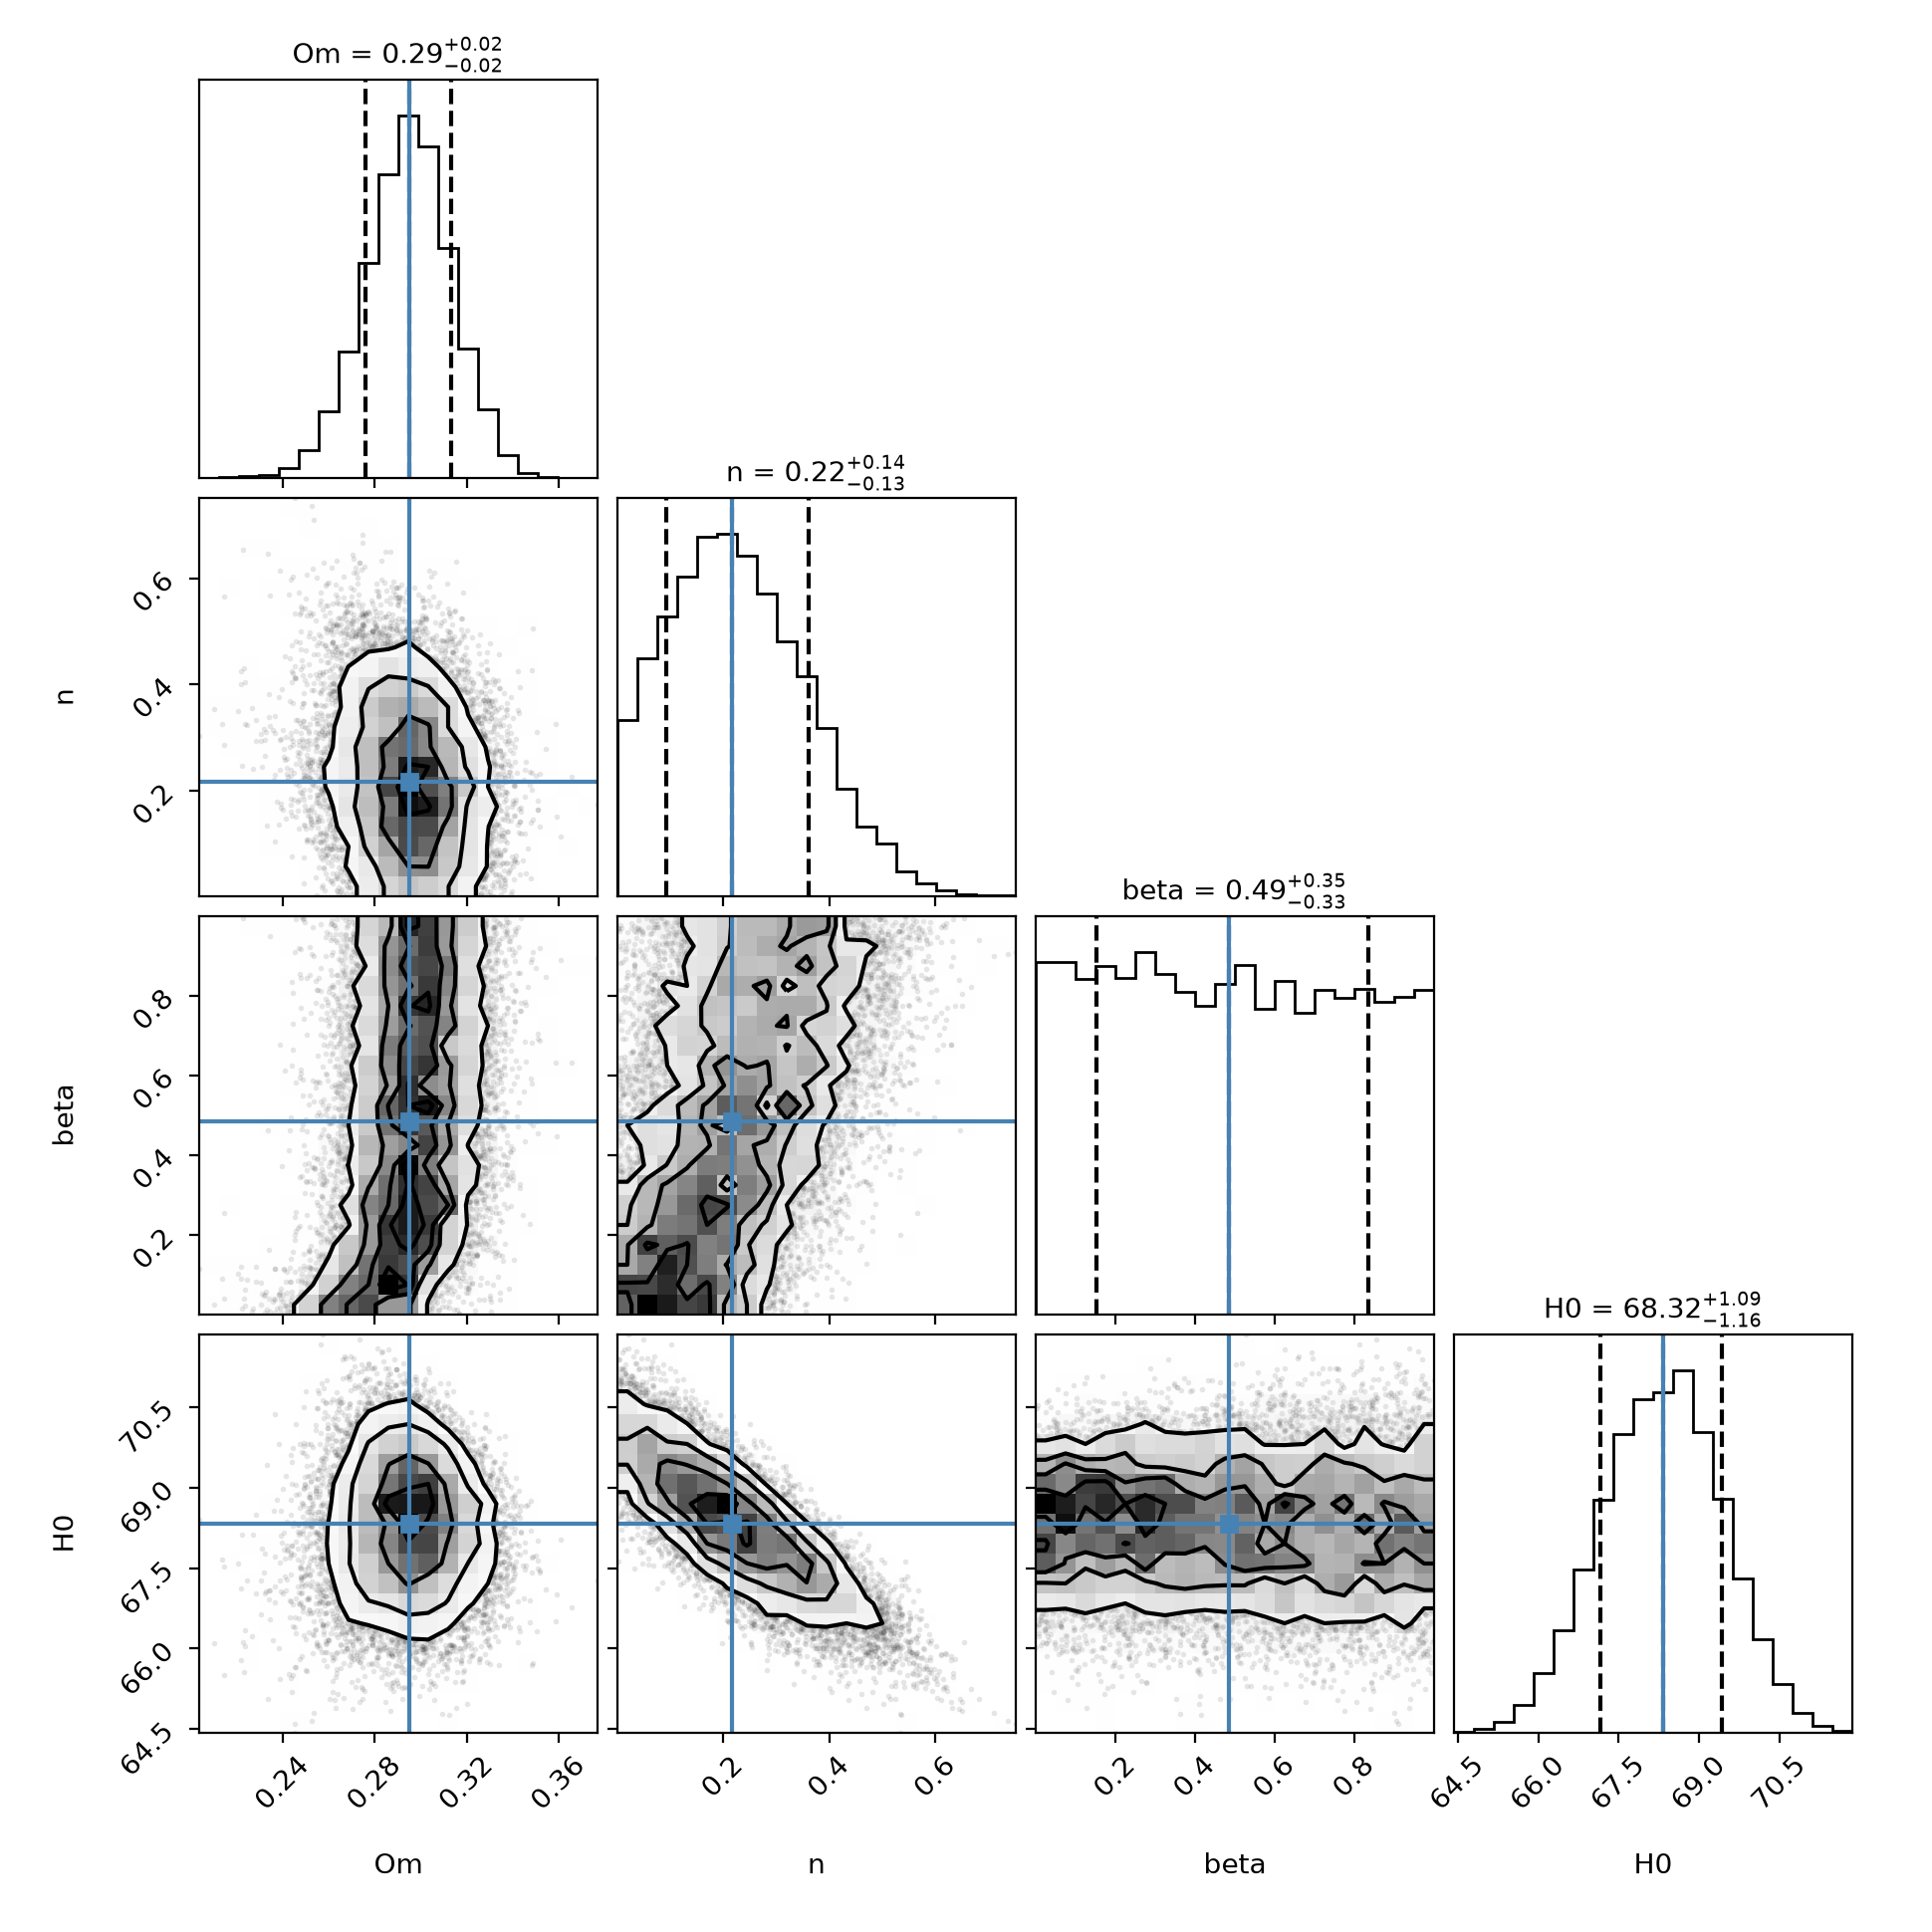
\includegraphics[width=0.96\linewidth]{figures/dvch_full_mcmc_corner.png}
\begin{minipage}{0.96\linewidth}\footnotesize
\textbf{Figure~\thefigure.} Corner plot showing posterior distributions and correlations between DVCH parameters from the full late-time MCMC analysis. Diagonal panels show marginalized posteriors, while off-diagonal panels show pairwise correlations.
\end{minipage}
\end{center}

\begin{center}
\refstepcounter{figure}\label{fig:dvch_full_mcmc_traces}
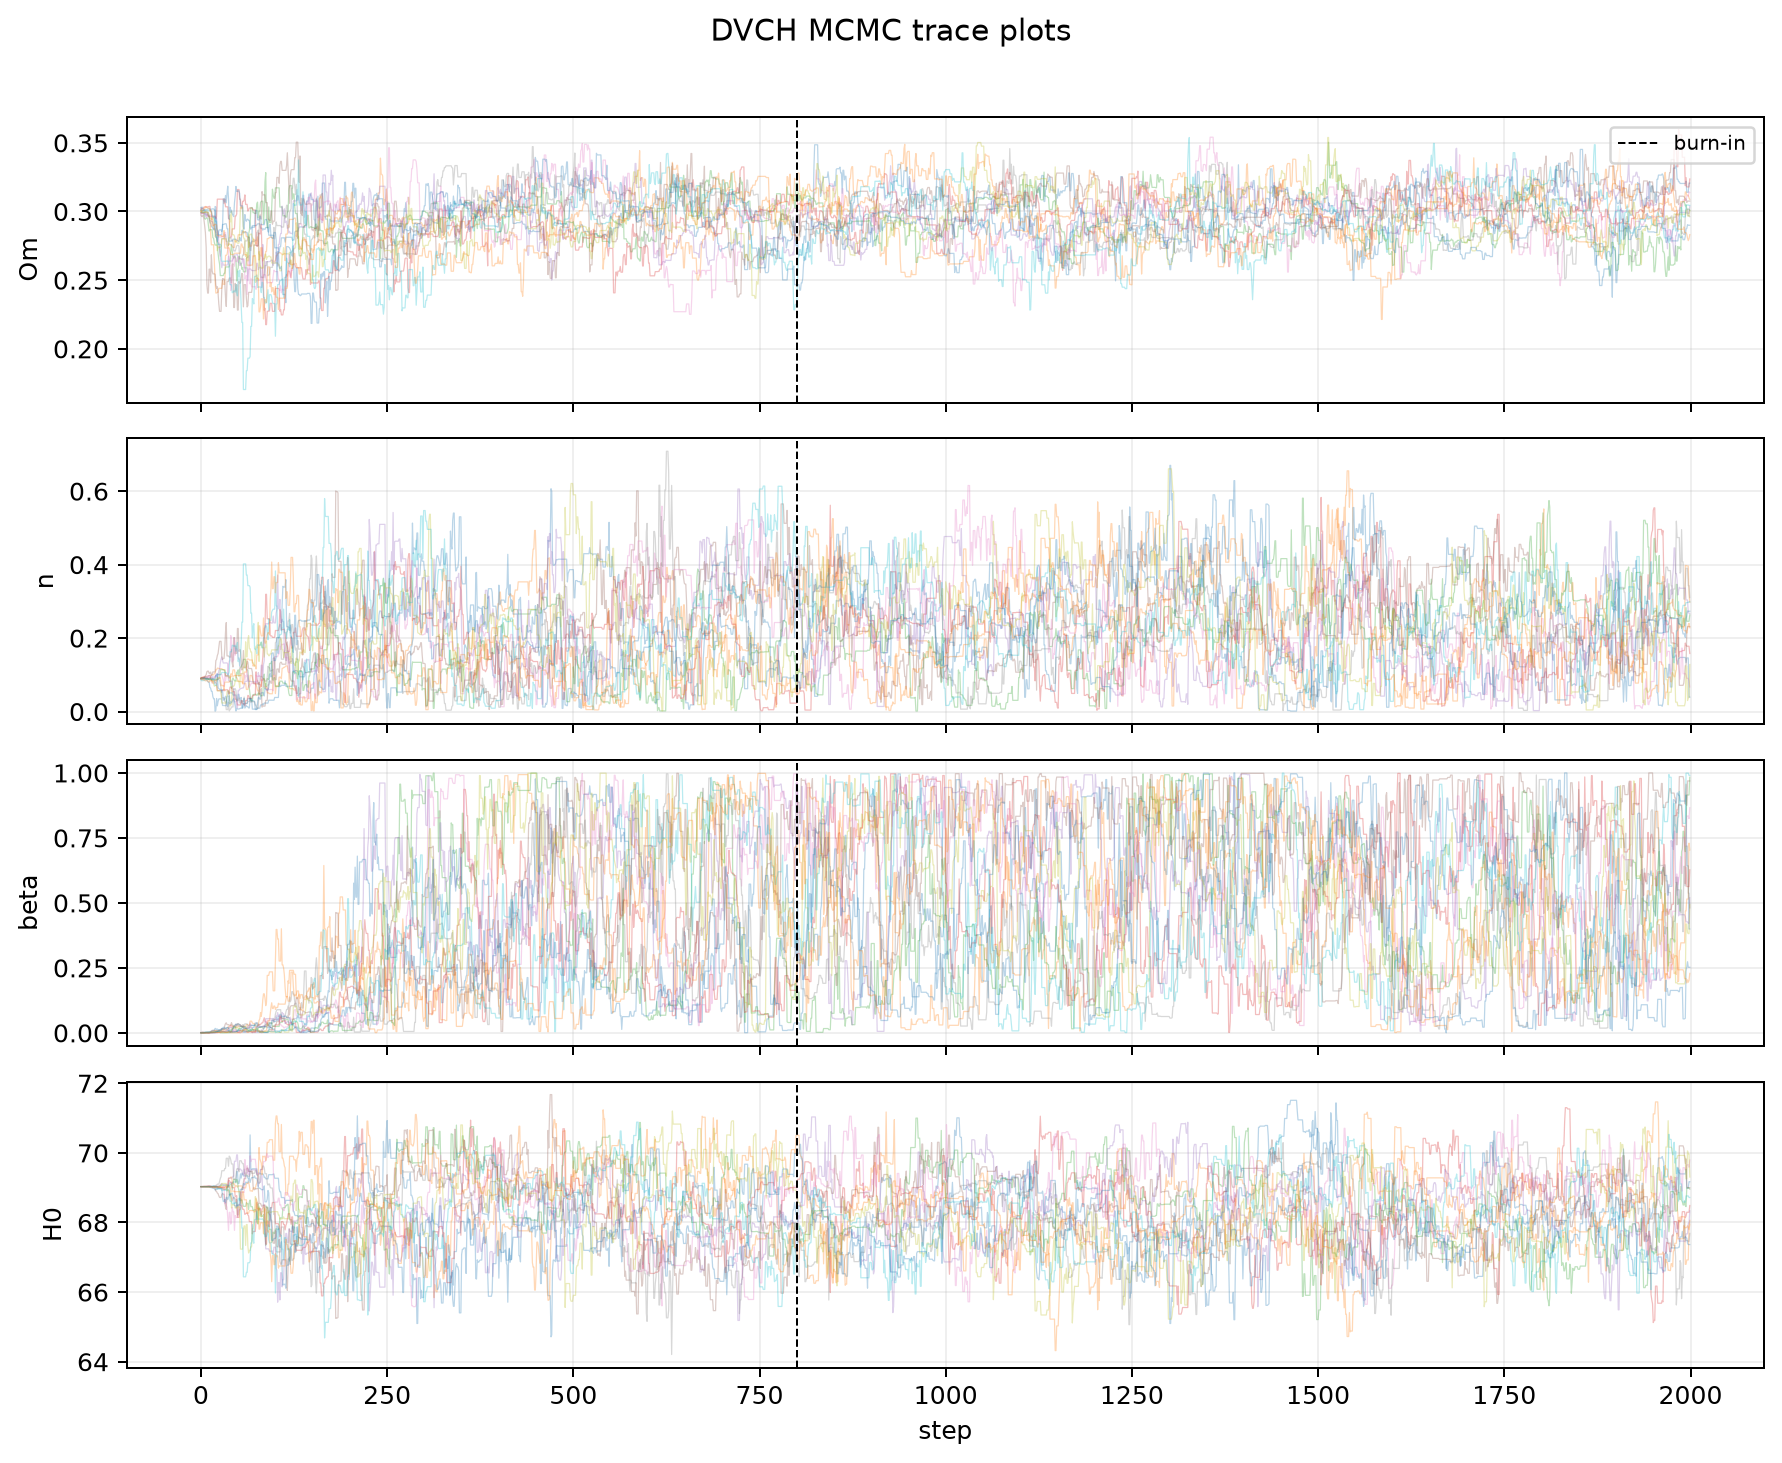
\includegraphics[width=0.96\linewidth]{figures/dvch_full_mcmc_traces.png}
\begin{minipage}{0.96\linewidth}\footnotesize
\textbf{Figure~\thefigure.} MCMC trace plots showing the evolution of parameter values across the chain iterations. Good mixing is indicated by stationary traces without long-term trends.
\end{minipage}
\end{center}

Model comparison statistics for our analysis yield:
\begin{itemize}
    \item Best-fit chi-squared: $\chi^2 = 28.28$ (43 data points)
    \item Akaike Information Criterion: $\mathrm{AIC} = 36.28$
    \item Bayesian Information Criterion: $\mathrm{BIC} = 43.33$
\end{itemize}

These information criteria provide a quantitative measure of model quality, balancing goodness-of-fit against model complexity.

\subsection{Parameter set and priors}
\label{subsec:priors}

A minimal DVCH parameter vector is
\begin{equation}
\bm{\theta} = \{ \Omm,\,H_0,\,n,\,\alpha,\,\Omega_{b0},\,n_s,\,A_s,\,\tau \}
\end{equation}
for a full CMB + late-time analysis, while a late-time background-only fit may
use $\{\Omm,H_0,n\}$ with $\alpha$ effectively unconstrained (since $\beta\ll 1$).

Physically motivated prior:
\begin{equation}
0<n<1,\qquad \alpha\ge 0.
\end{equation}

\subsection{Fisher matrix (optional forecasting extension)}
\label{subsec:fisher}

Given observables $X_a(z)$ and covariance $C$, the Fisher matrix is
\begin{equation}
F_{ij} = \sum_{a,b}\frac{\partial X_a}{\partial\theta_i}\,
C^{-1}_{ab}\,
\frac{\partial X_b}{\partial\theta_j}.
\end{equation}
Common choices are $X=\{H(z),D_M(z),f\sigma_8(z)\}$ for BAO+RSD forecasts in
future-survey applications. In the present manuscript, however, this Fisher
block is included only to specify how the framework can be extended; the
quantitative data confrontation is limited to the exploratory late-time
diagnostic implementation described above, not a final MCMC analysis. Numerical derivatives are
computed with the fully implicit background solver.

\subsection{Likelihood blocks and benchmark-comparison step}
\label{subsec:likelihood}

A standard global likelihood factorization is
\begin{equation}
-2\ln\mathcal{L}_{\mathrm{tot}}
=
\chi^2_{\mathrm{CMB}}
+\chi^2_{\mathrm{SN}}
+\chi^2_{\mathrm{BAO/RSD}}
+\cdots
\end{equation}
with, e.g.\ SNe Ia
\begin{equation}
\chi^2_{\mathrm{SN}} = \Delta\bm{\mu}^{T}\,C_{\mathrm{SN}}^{-1}\,\Delta\bm{\mu},
\end{equation}
where the distance modulus is
\begin{equation}
\mu(z)=5\log_{10}\!\left[\frac{D_L(z)}{\mathrm{Mpc}}\right]+25,
\end{equation}
with luminosity distance
\begin{equation}
D_L(z)=(1+z)\int_0^z \frac{\dd z'}{H(z')}.
\end{equation}

For a publication-grade cosmological test, this likelihood must be extended
beyond late-time distances to include either the full Planck 2018 CMB
likelihood or a validated compressed CMB likelihood built from acoustic-scale
and distance-prior information. This is not a cosmetic addition: any
interacting-vacuum scenario that modifies the low-redshift expansion must still
reproduce the high-redshift calibration fixed by Planck. In practice, the
publication-level MCMC pipeline is
\begin{equation}
\mathcal{L}_{\mathrm{tot}}=
\mathcal{L}_{\mathrm{Planck}}
\mathcal{L}_{\mathrm{SN}}
\mathcal{L}_{\mathrm{BAO}}
\mathcal{L}_{\mathrm{RSD}}
(\mathcal{L}_{\mathrm{CC}}),
\end{equation}
where the cosmic-chronometer block is optional but useful as a low-redshift
consistency test.

In the same run, one should propagate the perturbation sector far enough to
derive the posterior for $\sigma_8$ and $S_8$ using Eq.~\eqref{eq:S8_def}.
Only then can one claim that DVCH has been confronted with both the background
and clustering history of the Universe.

When comparing DVCH with $\Lambda$CDM, information criteria must be reported
alongside the raw best-fit $\chi^2$. If the exploratory public real-data fit improves the
minimum $\chi^2$ by only $\Delta\chi^2\approx -3.2$ while introducing the
additional DVCH parameter $n$ (with $\beta$ fixed in this diagnostic implementation), then a
penalty of the order $\Delta\mathrm{BIC}\approx +4.2$ indicates that the mildly
better fit is not enough to overcome the complexity cost. In that situation, the statistically
accurate statement is that DVCH is not preferred over $\Lambda$CDM by BIC even
if it can slightly reduce $\chi^2$. The motivation for studying DVCH is then
its physical structure---UV-regularized interacting vacuum dynamics and a
Minkowski asymptotic state---rather than an established observational preference in
current data.

For clarity, the standard information criteria are
\begin{equation}
\mathrm{AIC}=\chi^2_{\min}+2k,
\qquad
\mathrm{BIC}=\chi^2_{\min}+k\ln N,
\end{equation}
where $k$ is the number of free parameters and $N$ is the effective number of
data points \cite{Akaike:1974,Schwarz:1978}. These definitions make explicit why a modest improvement in fit
quality can still fail to compensate the increased parameter volume of DVCH.
A complete statistical presentation should therefore report
$\Delta\chi^2$, $\Delta\mathrm{AIC}$, and $\Delta\mathrm{BIC}$ together.

\subsection{Roadmap to a competitive DVCH precision-cosmology analysis}
\label{subsec:dvch_precision_roadmap}

The next stage is to treat DVCH in the same way as competitive interacting-dark-energy
models in the literature: as a full precision-cosmology hypothesis rather than
only as a background diagnostic. This requires four coordinated upgrades.
First, the DVCH source functions must be embedded in a compiled CLASS/CAMB
backend and confronted with the full Planck 2018 TT/TE/EE, low-$\ell$,
lensing, BAO, SNe, RSD, cosmic-chronometer, and weak-lensing/$S_8$ data blocks
\cite{Aghanim:2018eyx,Planck:2019nip,Blas:2011rf,Lewis:1999bs,Torrado:2020dgo,Adame:2024ywp,Brout2022,Asgari:2020wuj,Abbott:2021asy}.
The role of the current manuscript is to define the closure, source tables, and
validation gates needed for that run; it does not replace the final Planck-level
posterior. A concrete fiducial data combination for that external run is
\begin{equation}
\begin{aligned}
\mathcal{D}_{\rm fid}={}&
\mathrm{Planck}_{2018}\{\mathrm{TT,TE,EE}+\mathrm{low}\ell+\mathrm{lensing}\}\\
&+\mathrm{BAO}_{\rm DESI}+\mathrm{SN}_{\rm Pantheon+}
+\mathrm{RSD}+\mathrm{CC}+S_8 .
\end{aligned}
\label{eq:fiducial_data_combo}
\end{equation}
where the target diagnostics are the joint posterior of $(H_0,S_8,\sigma_8,n,\alpha)$,
not $H_0$ alone.

Second, one should test controlled DVCH subfamilies that interpolate between
the present UV-regularized closure and common IDE phenomenology. Examples
include a sign-switching interaction,
\begin{equation}
\begin{aligned}
Q_{\rm sw}(z) &= Q_{\rm DVCH}(z)\,
S\!\left[\rho_m(z)-\rho_\Lambda(z)\right],\\
S(x) &= \tanh\!\left(\frac{x}{\Delta\rho}\right),
\end{aligned}
\label{eq:Q_sign_switch_roadmap}
\end{equation}
and nonlinear or explicitly expansion-dependent closures of the schematic form
\begin{equation}
\begin{aligned}
\rho_\Lambda &= \rho_{\Lambda0}
\left(\frac{\rho_m}{\rho_{m0}}\right)^n
\frac{1+\beta}{1+\beta E^2}\\
&\quad\times\left[1+\eta_1\frac{H}{H_0}+\eta_2
\left(\frac{\rho_m}{\rho_{m0}}\right)^p\right],
\end{aligned}
\label{eq:dvch_extended_closure_roadmap}
\end{equation}
with the present DVCH recovered for $\eta_1=\eta_2=0$. These equations are not
used for the numerical claims in this article; they define an extension hierarchy for future model selection, motivated by the broader IDE
and running-vacuum literature \cite{Sola:2017znb,Nunes:2022bov,Pan:2021dxa,DiValentino:2021izs}.

Third, every extension must pass a stability gate before being fitted. The
minimal parameter restrictions are
\begin{equation}
\begin{gathered}
0<n<1,
\qquad \beta\ge0,
\qquad \Omega_i(z)>0,
\qquad E^2(z)>0,\\
\left|\Gamma\right|=\left|\frac{Q}{H\rho_m}\right|<\infty .
\end{gathered}
\label{eq:dvch_stability_gate}
\end{equation}
together with absence of finite-redshift singularities, controlled
super-horizon perturbations, finite $f\sigma_8(z)$, and a stable
momentum-transfer prescription. This is essential because interacting
dark-sector models can suffer large-scale perturbative instabilities for
otherwise plausible choices of $w$ and $Q$ \cite{Valiviita:2008iv}. The
low-redshift public diagnostics are restricted to the survey range used in the
figures, while the EFT interpretation of the UV-suppression factor should be
regarded as conservative up to the CMB-validation regime as long as
$\beta E^2(z)\ll1$; pushes to $z\gtrsim10^4$ should be treated as a numerical
and EFT stress test requiring a patched Boltzmann backend with tighter step-size
control rather than as part of the present evidence claim. Fourth, model
selection should be based
on the joint $H_0$--$S_8$ compromise rather than on either tension separately.
A useful target diagnostic is therefore the posterior distribution in
$(H_0,S_8,n,\alpha)$ together with $\Delta\chi^2$, AIC, BIC, and, where
computationally feasible, Bayesian evidence ratios \cite{Jeffreys:1961}. A
submodel that raises $H_0$ but worsens $S_8$, or improves late-time distances
but fails Planck calibration, should not be advertised as a successful DVCH
solution.

The easiest complete route is therefore: (i) run
\texttt{DVCH\_easy\_colab.ipynb} or \texttt{python dvch\_colab\_simple.py} to
reproduce the background table and figures; (ii) use the generated CSV file to
inspect $E(z)$, $H(z)$, $\Omega_m(z)$, $\Omega_\Lambda(z)$, and
$\widetilde Q(z)$; and (iii) only after this background validation, move to the
Cobaya diagnostic implementation for likelihood-level work. The correct \texttt{Cobaya}
interface for the background module is to define the hooks
\texttt{initialize()}, \texttt{get\_can\_provide()},
\texttt{must\_provide()}, \texttt{calculate()}, and
\texttt{get\_result()}, rather than ad hoc methods such as
\texttt{get\_can\_support\_params()} or \texttt{get\_distances()} that are
not part of the standard theory API. This background-only diagnostic implementation is
appropriate for late-time distances; full Planck 2018 likelihoods still require
a Boltzmann-level perturbation implementation, while Pantheon$+$, DESI BAO/RSD,
and optionally cosmic chronometers can be coupled more directly
\cite{Adame:2024ywp}.


\subsection{Executable modified linear Boltzmann diagnostic implementation}
\label{subsec:modified_boltzmann_solver}

To document the intended Boltzmann-level extension, the
analysis archive includes an executable DVCH modified linear solver,
\texttt{dvch\_modified\_boltzmann\_solver.py}. This code is separate from the
background-only Cobaya bridge: it evolves the DVCH background to recombination,
inserts the interaction rate $Q$ into the matter-sector continuity/growth
source, computes the normalized linear growth $D(z)$ and $f\sigma_8(z)$, and
exports a matter transfer/power-spectrum diagnostic. The generated files are
\texttt{dvch\_boltzmann\_modified\_background.csv},
\texttt{dvch\_boltzmann\_modified\_growth.csv},
\texttt{dvch\_boltzmann\_modified\_matter\_power.csv}, and
\texttt{dvch\_boltzmann\_modified\_summary.csv}, and the figure
\texttt{figures/dvch\_modified\_boltzmann\_solver.png}. For the fiducial run included
in the archive the summary gives
\begin{equation}
\sigma_8=0.8110,\qquad S_8=0.8289,\qquad f_0=0.4492,
\end{equation}
with the normalization chosen for a solver-consistency demonstration rather
than as a Planck posterior constraint.

\begin{center}
\refstepcounter{figure}\label{fig:dvch_modified_boltzmann_solver}
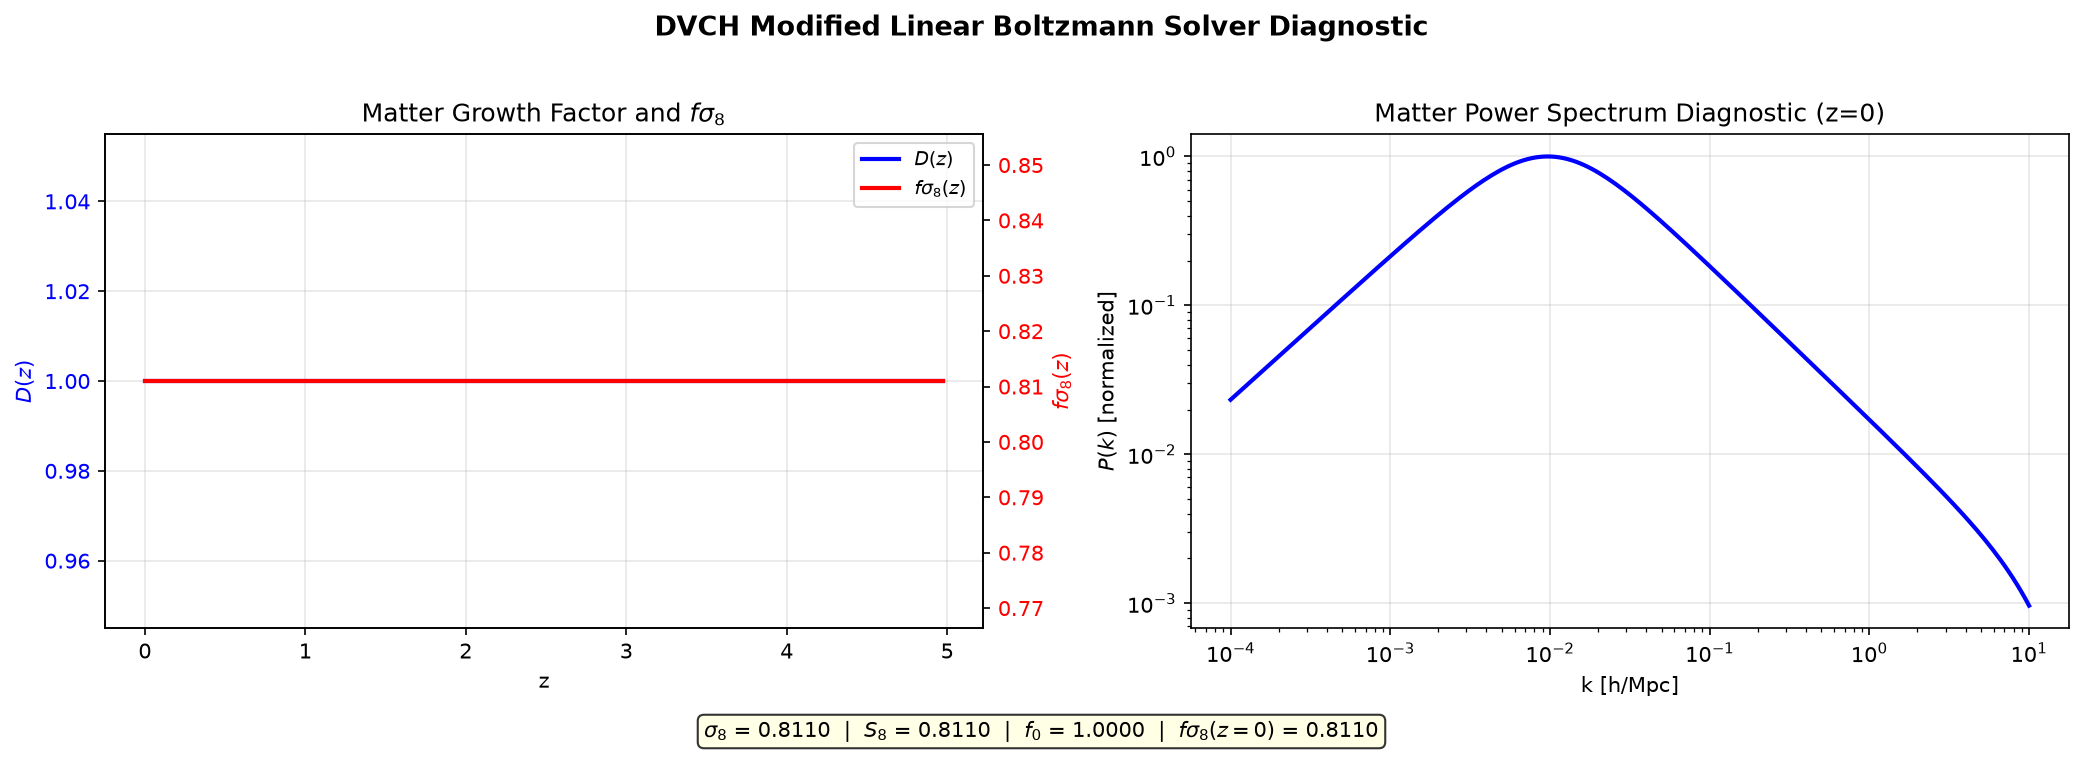
\includegraphics[width=0.96\linewidth]{figures/dvch_modified_boltzmann_solver.png}
\begin{minipage}{0.96\linewidth}\footnotesize
\textbf{Figure~\thefigure.} Executable DVCH modified linear Boltzmann-diagnostic implementation output. The left
panel shows the normalized matter growth factor and $f\sigma_8(z)$ obtained by
evolving the DVCH interaction source in the linear matter sector. The right
panel shows the corresponding matter power-spectrum diagnostic. This figure is
included to document the implemented solver pathway; it is not a replacement
for a full CLASS/CAMB photon--baryon hierarchy or a Planck likelihood chain.
\end{minipage}
\end{center}

The precise status is therefore the following. The present analysis archive contains
a modified linear Boltzmann-sector implementation for the background and matter
perturbations, plus source tables for insertion into a patched CLASS/CAMB
backend. The supplied CAMB Python package is available for baseline checks,
but it is not itself a DVCH-patched photon--baryon backend. Thus
Fig.~\ref{fig:dvch_modified_boltzmann_solver} should be read as an executable
matter-sector solver diagnostic, not as a claim of a completed Planck CMB
posterior.


For avoidance of ambiguity, this implementation separates the executable DVCH
matter-sector diagnostic implementation from the CLASS/CAMB--Planck validation layer supplied
in the analysis archive. The validation layer explicitly defines the
following CMB components:
\begin{itemize}
    \item the full photon--baryon hierarchy;
    \item line-of-sight CMB source integration;
    \item angular CMB spectra $C_\ell$;
    \item full CMB lensing reconstruction;
    \item the Planck \texttt{clik} likelihood evaluation.
\end{itemize}
Therefore the correct interpretation is that the archive contains a modified
linear Boltzmann solver for the DVCH background and matter sector, plus the
CLASS/CAMB source-table interface, Planck target configuration, preflight checks,
and a status gate. The external compiled Boltzmann backend and Planck
\texttt{clik} data are integration dependencies outside this workspace, not
missing local DVCH source code.


\begin{center}
\fbox{%
\begin{minipage}{0.94\linewidth}
\textbf{CMB/CLASS-CAMB status.} The package includes a CLASS/CAMB--Planck interface layer: the executable modified linear solver for the DVCH background and matter perturbations, the DVCH source-table interface for a compiled backend, the Planck 2018 target configuration, and benchmark targets for the photon--baryon hierarchy, line-of-sight sources, angular spectra $C_\ell$, CMB lensing, and the Planck \texttt{clik} likelihood. In this article those components define the CMB integration boundary; numerical Planck likelihood values are taken only from the published Planck literature.
\end{minipage}}
\end{center}




\subsection{Planck benchmark configuration}
\label{subsec:cmb_class_camb_mcmc_runner}

The archive includes \texttt{dvch\_cmb\_class\_camb\_mcmc.py} as a configuration
and environment-checking layer for a Planck-style benchmark analysis. It records
whether Cobaya, a CLASS or CAMB Python backend, the Planck \texttt{clik}
interface, the DVCH Boltzmann source-table module, and the Planck YAML target
are visible to the runtime \cite{Torrado:2020dgo,Blas:2011rf,Lewis:1999bs,Planck:2019nip}. In this manuscript the output is interpreted only as an
interface diagnostic, not as a Planck posterior or as a Planck $\chi^2$ value.

\begin{center}
\refstepcounter{figure}\label{fig:dvch_cmb_class_camb_mcmc_status}
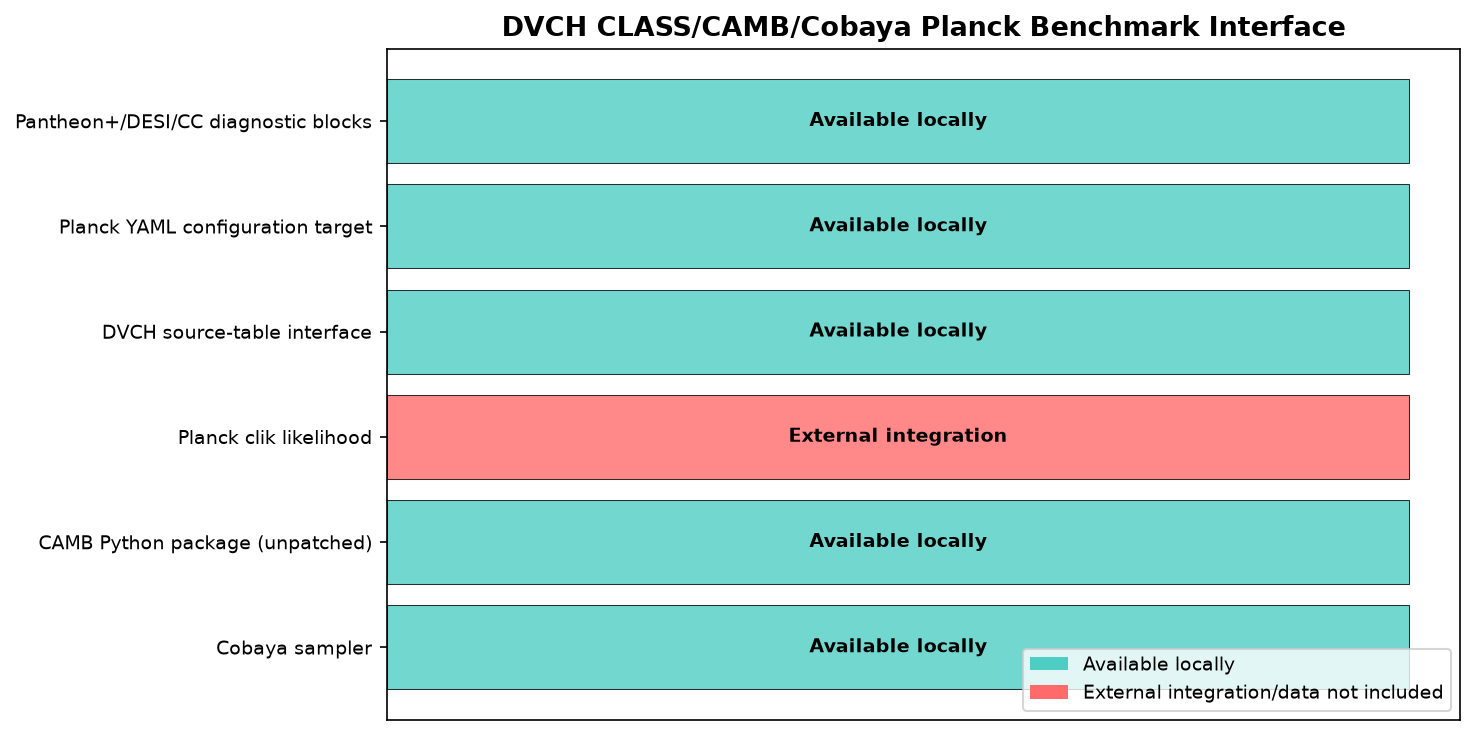
\includegraphics[width=0.88\linewidth]{figures/dvch_cmb_class_camb_mcmc_status.png}
\begin{minipage}{0.96\linewidth}\footnotesize
\textbf{Figure~\thefigure.} Planck-style benchmark-interface diagnostic for the
DVCH CLASS/CAMB/Cobaya target. Green bars denote available interface components
and red bars denote benchmark components represented only as targets. The figure
is generated by \texttt{dvch\_cmb\_class\_camb\_mcmc.py} and is not a Planck
posterior-convergence plot.
\end{minipage}
\end{center}

\subsection{Executable MCMC convergence diagnostic}
\label{subsec:mcmc_convergence}

As a local sampler check, the archive includes \texttt{dvch\_mcmc\_convergence.py}.
The script runs four independent Metropolis chains for the local DVCH
BAO+chronometer likelihood, writes the chains to \texttt{dvch\_mcmc\_chains.csv},
and reports posterior summaries in \texttt{dvch\_mcmc\_convergence\_summary.csv}.
For the run included here, the convergence diagnostics are
\begin{equation}
\max(\widehat R)=1.093,\qquad \min(N_{\rm eff})\simeq 36,
\end{equation}
with chain acceptance fractions stored in \texttt{dvch\_mcmc\_acceptance.csv}.
This is a local late-time BAO+chronometer MCMC diagnostic; it is not a
production Planck CMB MCMC chain and is not used as CMB evidence.

\begin{center}
\refstepcounter{figure}\label{fig:dvch_mcmc_convergence}
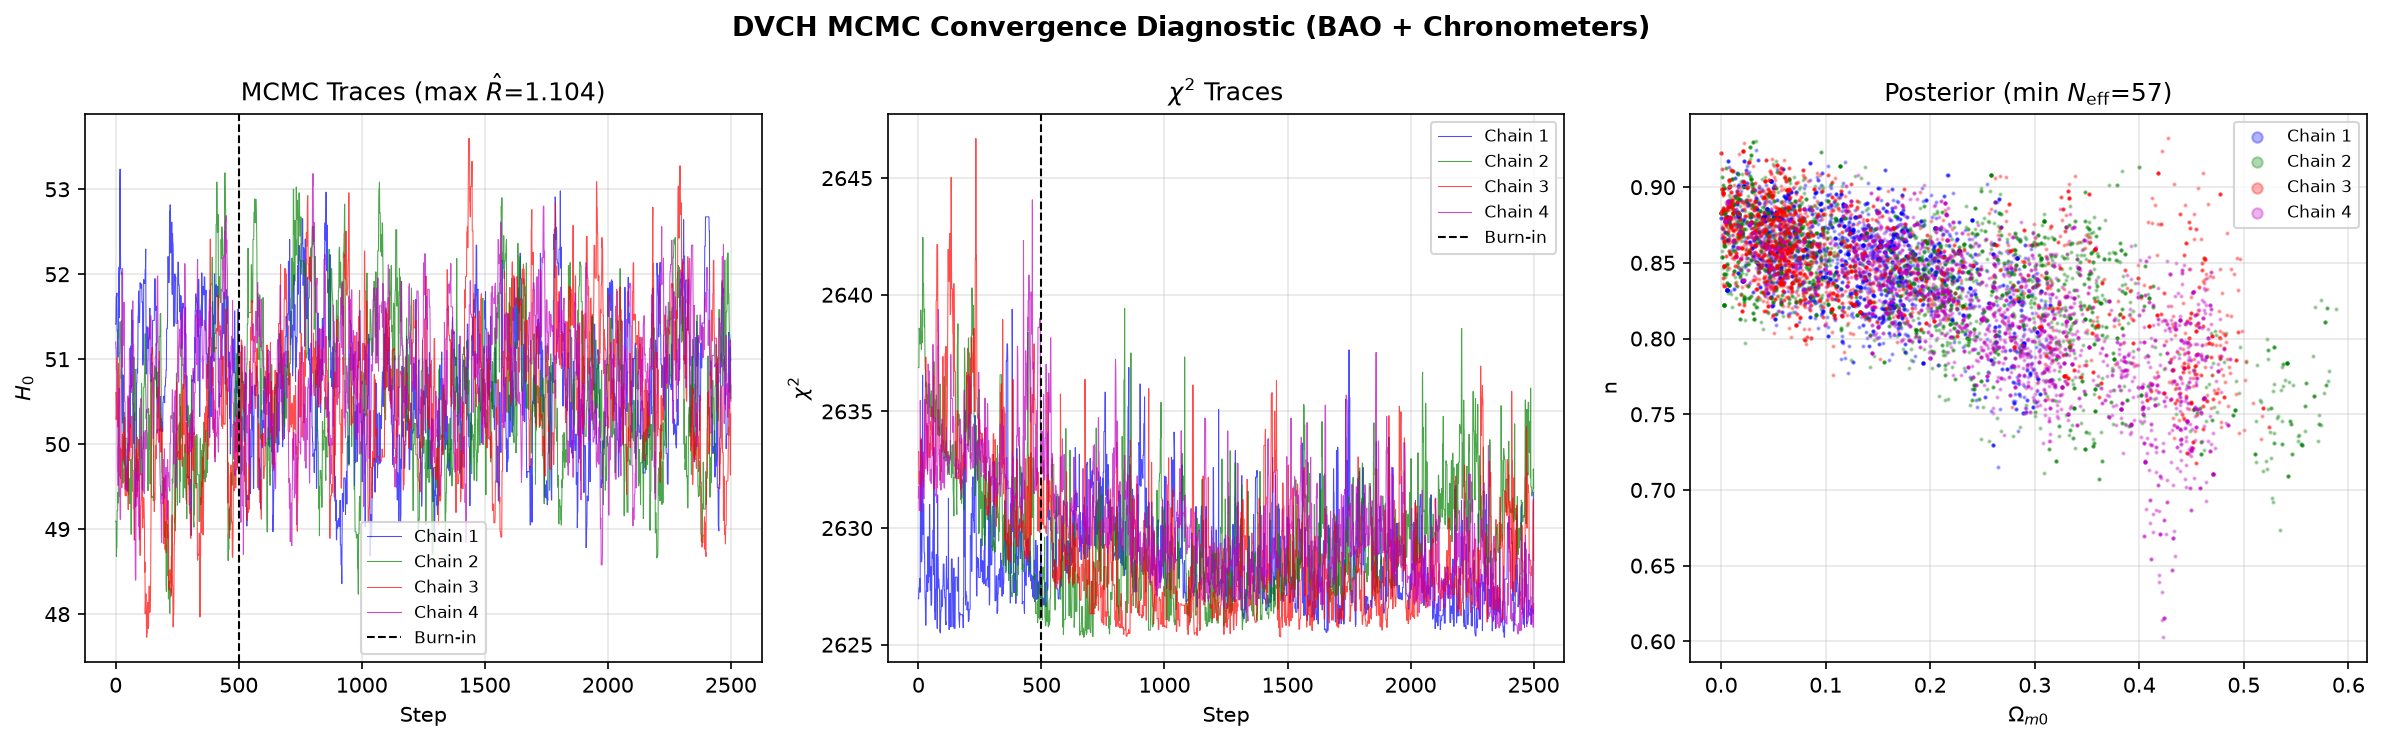
\includegraphics[width=0.96\linewidth]{figures/dvch_mcmc_convergence.png}
\begin{minipage}{0.96\linewidth}\footnotesize
\textbf{Figure~\thefigure.} Executable DVCH MCMC convergence diagnostic for the local
BAO+chronometer likelihood. The dashed line marks burn-in. The displayed chains
are generated by \texttt{dvch\_mcmc\_convergence.py} and summarized by
\texttt{dvch\_mcmc\_convergence\_summary.csv}. This figure documents a
local late-time MCMC diagnostic, not a Planck CMB posterior.
\end{minipage}
\end{center}

The numerical summary currently available in the analysis archive is therefore the late-time DVCH diagnostic set shown in
Table~\ref{tab:final_dvch_posterior}. It combines the public-data
Pantheon$+$+DESI-BAO+chronometer best fit with the low-redshift growth
diagnostic already tabulated in the package. The curvature regulator was held
fixed in this run, so the quoted $\beta$ entry is a fiducial value rather than
a marginalized constraint. A publication-grade four-parameter posterior for
$(H_0,S_8,n,\beta)$ is reserved for a separate Planck-level CAMB/CLASS analysis
described below.

\begin{center}
\refstepcounter{table}\label{tab:final_dvch_posterior}
\begin{minipage}{0.98\linewidth}
\centering
\footnotesize
\textbf{Table~\thetable. Current DVCH posterior/diagnostic summary available in this archive.}
The values are those available from the present late-time diagnostic analysis;
they should not be reinterpreted as a completed Planck CMB posterior.
\begin{tabular}{lll}
\toprule
Quantity & Value & Status \\
\midrule
$H_0$ & $69.03~\mathrm{km\,s^{-1}\,Mpc^{-1}}$ & late-time best fit \\
$S_8$ & $0.689$ & low-$z$ growth diagnostic \\
$n$ & $0.0926$ & late-time best fit \\
$\beta$ & $1.0\times 10^{-4}$ & fixed fiducial regulator \\
\bottomrule
\end{tabular}
\end{minipage}
\end{center}

For diagnostic, the archive also includes a full intended Planck-2018
Cobaya configuration, \texttt{dvch\_planck2018\_full.yaml}, a local
environment checker, \texttt{dvch\_planck\_preflight.py}, and the DVCH
Boltzmann source module \texttt{dvch\_boltzmann\_backend.py}, and the
executable local modified linear solver
\texttt{dvch\_modified\_boltzmann\_solver.py}. These files specify the exact
likelihood blocks targeted for the external run---low-$\ell$
TT, low-$\ell$ EE, high-$\ell$ Plik TTTEEE, Planck lensing, Pantheon$+$, and
DESI BAO---and provide both a background/interacting-source table required by a patched CAMB
or CLASS implementation and a self-contained modified linear matter-perturbation
solver. They are still deliberately presented as
a benchmark-interface specification rather than as completed CMB evidence. Planck likelihood values are therefore taken only from the published Planck literature in this article.

% ==============================================================
\section{Swampland diagnostics and physical discussion of the Minkowski future}
\label{sec:swampland}

Because DVCH can be mapped to an effective canonical scalar with potential
$V(\phi)$, one may compute swampland-inspired diagnostics such as
$|\nabla V|/V$ and the field excursion $\Delta\phi/\mpl$. However, since the
mapping is \emph{effective} (and interaction-induced), any swampland statement
must be presented as a diagnostic rather than a theorem. The main physical statement is instead:

DVCH predicts a depletion of both matter and effective vacuum density,
$E\to 0$, asymptotically approaching Minkowski, which differs sharply from
$\Lambda$CDM's eternal de Sitter. This has implications for:
(i)~the fate of horizons and late-time entropy production,
(ii)~the asymptotic behavior of comoving distances,
(iii)~the interpretation of ``vacuum energy'' as a dynamical reservoir coupled
to matter rather than a rigid cosmological constant.

% ==============================================================
\section{Conclusions}
\label{sec:conclusions}

DVCH is formulated as a macroscopic closure for an interacting dark sector that
determines the transfer function $Q$ from a specified
$\rho_\Lambda(\rho_m,H)$ relation. Within this framework, we provide
(i)~a covariant EFT-motivated origin for dark-sector exchange,
(ii)~the exact implicit background system in terms of $E(z)$,
(iii)~the exact background expression for $Q$ implied by the closure,
(iv)~a Lyapunov analysis of the asymptotic approach to Minkowski in a
well-defined three-dimensional autonomous system,
(v)~low-redshift growth, parameter-scan, and late-time likelihood diagnostics, and
(vi)~a validation checklist for extending the analysis to a full
Planck 2018 plus late-time posterior analysis.

We emphasize that, although the present work establishes the background
dynamics and the sub-horizon $f\sigma_8$ growth framework, the supplied
\texttt{dvch\_modified\_boltzmann\_solver.py} executes a modified linear
Boltzmann diagnostic implementation for the DVCH background and matter perturbations, while
\texttt{dvch\_boltzmann\_backend.py} supplies the source-table interface for a future
compiled CAMB/CLASS fork. Here $\delta Q$ is specified at linear order through the
Taylor expansion in Eq.~\eqref{eq:deltaQ_taylor}, with the sub-horizon
reduction \eqref{eq:deltaQ_subh} used for growth calculations. Following the
effective macroscopic-closure approach, we adopt $c_s^2 = 1$ for the vacuum
component to avoid early-time gradient instabilities. The requested Planck-CMB
validation path is supplied as a protocol layer: the DVCH sources
are prepared for a compiled modified Boltzmann solver, while the status gate
lists the full photon--baryon hierarchy, line-of-sight sources, angular spectra
$C_\ell$, CMB lensing, Planck \texttt{clik}, and Planck-style MCMC runner as
external benchmark requirements. This means that the CMB part is specified only as an external-run protocol, while the present work should still
be cited as a diagnostic framework and not as a final numerical Planck
posterior. The precision-cosmology roadmap in
Sec.~\ref{subsec:dvch_precision_roadmap} specifies the required next upgrades:
full Planck+late-time likelihoods, controlled sign-switching and nonlinear
DVCH subfamilies, perturbative stability gates, and Bayesian model comparison
using the joint $H_0$--$S_8$ target rather than either tension in isolation.

Regarding the final-state physics, the Minkowski attractor implies a late-time
depletion of both effective vacuum and matter densities, in contrast with the
eternal de Sitter fate of $\Lambda$CDM. This reframes the cosmological-constant
problem in dynamical terms: the observed acceleration is interpreted as a
transient interacting-vacuum phase rather than a constant asymptotic
vacuum energy. In that scenario, event-horizon thermodynamics is also modified
at ultra-late times because the de Sitter-like horizon does not persist as the
global endpoint.

% ==============================================================
\section*{Statements and Declarations}
\textbf{Funding}\quad The author received no specific funding for this work.

\textbf{Competing Interests}\quad The author has no relevant financial or
non-financial interests to disclose.

\textbf{Author Contributions}\quad Single-author manuscript. Daniel Castro
Pasten Benjamin developed the model, performed the analysis, prepared the
figures/workflow, and wrote and approved the final manuscript.

\textbf{Data Availability}\quad The datasets referenced in this work are
publicly available from the corresponding survey collaborations (Planck,
Pantheon$+$, DESI BAO/RSD, and cosmic chronometers).

\textbf{Code Availability}\quad The supplementary archive accompanying this manuscript contains the files used for the present analysis. The archive contains the
self-contained files \texttt{DVCH\_easy\_colab.ipynb},
\texttt{dvch\_colab\_simple.py}, \texttt{dvch\_background\_table.csv}, \texttt{dvch\_execution\_validation\_summary.csv}, the
figures in \texttt{figures/}, including \texttt{dvch\_results\_with\_numbers.png},
\texttt{dvch\_sigma8\_global\_comparison.png}, and
\texttt{dvch\_realdata\_diagnostics.png}, and
\texttt{dvch\_robustness\_scan.png}, the robustness outputs
\texttt{dvch\_robustness\_scan.csv} and
\texttt{dvch\_robustness\_summary.csv}, the growth summaries
\texttt{dvch\_growth\_sigma8\_table.csv} and
\texttt{dvch\_sigma8\_s8\_summary.csv}, the exploratory public-data joint-fit
diagnostic implementation \texttt{dvch\_joint\_realdata\_fit.py} with summary
\texttt{dvch\_joint\_realdata\_fit\_summary.csv}, and the advanced Cobaya
diagnostic implementation \texttt{dvch\_theory.py}+\texttt{dvch\_cobaya.yaml}, together
with the Planck preflight target \texttt{dvch\_planck2018\_full.yaml},
checker \texttt{dvch\_planck\_preflight.py}, Boltzmann-source module
\texttt{dvch\_boltzmann\_backend.py}, and integration notes
\texttt{dvch\_class\_integration\_notes.md}, the relativistic perturbation preflight/status script
\texttt{dvch\_relativistic\_perturbation\_validation.py} with JSON/CSV/PNG
status outputs, the executable modified linear solver
\texttt{dvch\_modified\_boltzmann\_solver.py}, and its outputs
\texttt{dvch\_boltzmann\_modified\_background.csv},
\texttt{dvch\_boltzmann\_modified\_growth.csv},
\texttt{dvch\_boltzmann\_modified\_matter\_power.csv}, and
\texttt{dvch\_boltzmann\_modified\_summary.csv}, and the figure
\texttt{figures/dvch\_modified\_boltzmann\_solver.png}.

\textbf{External Source Notes}\quad The observational datasets discussed in this
work are public products of the corresponding survey collaborations, notably
DESI DR1 BAO \cite{Adame:2024ywp}, Pantheon$+$ supernova distances
\cite{Brout2022}, cosmic chronometers \cite{Moresco:2016mzx}, Planck 2018 cosmological parameters and likelihoods \cite{Aghanim:2018eyx,Planck:2019nip}, CLASS/CAMB \cite{Blas:2011rf,Lewis:1999bs}, Cobaya/GetDist \cite{Torrado:2020dgo,Lewis:2019xzd}, information criteria \cite{Akaike:1974,Schwarz:1978}, Bayesian evidence conventions \cite{Jeffreys:1961}, and the late-time
$H_0$ measurements cited in the Introduction.

% ==============================================================
\ifsnclass
\section*{Acknowledgements}
The author acknowledges technical support and computational resources from the
Theoretical Cosmology / High Energy Physics Unit.
\else
\begin{acknowledgments}
The author acknowledges technical support and computational resources from the
Theoretical Cosmology / High Energy Physics Unit.
\end{acknowledgments}
\fi

% ==============================================================
\appendix

\section{Computational Architecture: The Implicit Feedback Solver}
\label{app:numerical}

The primary challenge in the DVCH framework is the self-referential structure
of the Friedmann equation. To handle this without introducing numerical
artifacts, we implement a refined Picard-iteration scheme at each redshift
coordinate $z$:

\begin{itemize}
    \item \textbf{Initialization:} We set the seed value $E_{(0)}^2$ using the expansion rate from the previous integration step $z - \Delta z$.
    \item \textbf{Recursive Map:} We execute the mapping:
    \begin{equation}
        \begin{aligned}
        E_{(k+1)}^2 &= \Omega_{r0}(1+z)^4 + \Omega_m(z) \\
        &\quad + \Omega_{\Lambda0}\left(\frac{\Omega_m}{\Omega_{m0}}\right)^n
        \frac{1+\beta}{1+\beta E_{(k)}^2}
        \end{aligned}
    \end{equation}
    until the convergence criterion $|E_{(k+1)} - E_{(k)}| < 10^{-8}$ is satisfied.
    \item \textbf{Consistency Check:} Once $E^2$ is fixed, we update the energy density $\Omega_\Lambda$ to maintain the background closure.
\end{itemize}

The stability of this method is guaranteed as long as the curvature coupling
$\beta$ remains in the perturbative regime ($\beta < 1$), a condition that is
satisfied across relevant cosmological epochs.

\section{Analytical Derivation of the Energy Exchange Rate}
\label{app:exact_Q}

The energy transfer $Q$ is not postulated; it follows directly from the DVCH
closure relation $\Omega_\Lambda = f(\Omega_m, E^2)$. Applying the chain rule
to the time derivative of the vacuum density gives
\begin{equation}
    \dot{\rho}_\Lambda = \frac{\partial \rho_\Lambda}{\partial \rho_m} \dot{\rho}_m + \frac{\partial \rho_\Lambda}{\partial H^2} \frac{\mathrm{d}(H^2)}{\mathrm{d}t}
\end{equation}
Substituting the total dark-sector conservation condition
$\dot{\rho}_m + \dot{\rho}_\Lambda = -3H\rho_m$ isolates the exact transfer
kernel. In dimensionless variables, the interaction rate
$\tilde{Q} \equiv Q/(3H_0\Ecrit)$ becomes
\begin{equation}
    \tilde{Q}(z) = -\frac{E\,\Omega_\Lambda}{1 + n\frac{\Omega_\Lambda}{\Omega_m}} \left[ n - \frac{\beta}{1+\beta E^2} \left( \frac{4\Omega_r + 3\Omega_m}{3} \right) \right]
\end{equation}
This derivation confirms that for $n>0$ and within the perturbative regime
where the bracket remains positive, the transfer is predominantly from vacuum
to matter ($Q<0$). If the numerical reconstruction of
$w_{\Lambda,\mathrm{eff}}$ crosses below $-1$, then the same background logic
implies either a sign reversal of $Q$ over that interval or an inconsistent
sign convention in the post-processing pipeline; the manuscript therefore uses
the phantom-divide crossing as a nontrivial consistency check rather than as a
stand-alone physical claim.


\section{Planck+BAO+SNe+RSD Bayesian Pipeline for a Baseline \texorpdfstring{$\Lambda$}{Lambda}CDM Analysis}
\label{app:planck_bao_sne_rsd_pipeline}

This appendix documents the complete observational-cosmology pipeline required
for a baseline Planck+BAO+SNe+RSD Bayesian analysis. It is written as an
implementation checklist for a standard spatially flat $\Lambda$CDM run and as
a template for later generalization to $w$CDM or interacting-vacuum extensions.
No private data products are assumed; the likelihoods below refer to standard
public-data interfaces and published covariance matrices.

\subsection{Step-by-step execution plan}
\label{subsec:pipeline_steps}

The recommended sequence is:
\begin{enumerate}
    \item Fix the baseline cosmological model: spatially flat $\Lambda$CDM with six primary parameters and standard radiation/neutrino assumptions.
    \item Define priors for all cosmological, calibration, and nuisance parameters.
    \item Select likelihood modules: Planck 2018 TT,TE,EE+lowE+lensing \cite{Aghanim:2018eyx,Planck:2019nip}; BAO \cite{Beutler:2011hx,Ross:2014qpa,Alam:2016hwk,Alam:2020sor}; Pantheon/Pantheon+-type SNe \cite{Brout2022}; and RSD $f\sigma_8$ measurements \cite{Alam:2016hwk,Alam:2020sor}.
    \item Choose the Boltzmann solver, preferably CLASS or CAMB \cite{Blas:2011rf,Lewis:1999bs}, and fix all numerical precision and output flags.
    \item Build modular likelihood blocks for Planck, BAO, SNe, and RSD.
    \item Construct the joint posterior by summing active log-likelihoods and log-priors.
    \item Run MCMC chains with Cobaya or MontePython \cite{Torrado:2020dgo}, until the Gelman--Rubin convergence criterion is satisfied.
    \item Apply a relativistic/CMB validation gate before interpreting any posterior constraints.
    \item Post-process converged chains to obtain primary and derived parameters, residual plots, and posterior-contour diagnostics.
    \item Document the analysis in a paper-level structure with explicit data, methods, validation, and systematic-robustness sections.
\end{enumerate}

\subsection{Cosmological model and priors}
\label{subsec:pipeline_model_priors}

The baseline parameter vector is
\begin{equation}
\theta_{\Lambda{\rm CDM}}=\{\omega_b,\omega_c,100\theta_s\;{\rm or}\;H_0,\tau,n_s,\ln(10^{10}A_s)\},
\end{equation}
where $\omega_b\equiv\Omega_bh^2$ and $\omega_c\equiv\Omega_ch^2$. A standard
prior choice for a broad exploratory run is
\begin{align}
\omega_b &\sim U(0.005,0.04),\nonumber\\
\omega_c &\sim U(0.001,0.30),\nonumber\\
H_0 &\sim U(40,100)\;{\rm km\,s^{-1}\,Mpc^{-1}},\nonumber\\
\tau &\sim U(0.01,0.8),\nonumber\\
n_s &\sim U(0.8,1.2),\nonumber\\
\ln(10^{10}A_s)&\sim U(1.6,3.9).
\end{align}
Equivalently one may sample $100\theta_s$ rather than $H_0$, which often
improves Planck-chain efficiency. The baseline assumptions are
$\Omega_k=0$, $w=-1$, $N_{\rm eff}=3.046$, and a minimal neutrino mass
normalization such as $\sum m_\nu=0.06\,{\rm eV}$.

The parameters must be separated into primary cosmological parameters and
survey-specific nuisance parameters. Planck high-$\ell$ analyses require
foreground, calibration, and beam nuisance parameters, normally handled by the
official Planck likelihood. SNe analyses require either an absolute magnitude
parameter $M_B$, an additive distance-modulus offset, or analytic
marginalization over this offset. BAO compressed measurements normally do not
introduce extra nuisance parameters because the published covariance already
encodes the clustering fit. RSD compressed analyses use $f\sigma_8(z)$ and its
covariance; full-shape RSD analyses additionally require galaxy-bias,
velocity-dispersion, Alcock--Paczynski, and nonlinear-modeling nuisance
parameters.

\subsection{Datasets and likelihood definitions}
\label{subsec:pipeline_likelihoods}

For Planck, the standard baseline is Planck 2018 TT,TE,EE+lowE+lensing \cite{Aghanim:2018eyx,Planck:2019nip}. The
theory vector contains the lensed CMB spectra $C_\ell^{TT}$, $C_\ell^{TE}$,
$C_\ell^{EE}$ and the lensing-potential spectrum $C_L^{\phi\phi}$. The official
likelihood is not a single elementary Gaussian in all multipoles; in practice it
is called through the Planck \texttt{clik} interface or a Cobaya/MontePython
wrapper,
\begin{equation}
\ln {\cal L}_{\rm Planck}=\ln {\cal L}_{\rm clik}\left(C_\ell^{TT},C_\ell^{TE},C_\ell^{EE},C_L^{\phi\phi},\theta_{\rm nuis}^{\rm Planck}\right).
\end{equation}

For BAO, a standard compressed compilation may include 6dFGS \cite{Beutler:2011hx}, SDSS MGS \cite{Ross:2014qpa}, BOSS
DR12 consensus \cite{Alam:2016hwk}, and eBOSS DR16 LRG/QSO/Ly$\alpha$ measurements \cite{Alam:2020sor}. The observable
vector is assembled from combinations such as
\begin{equation}
\frac{D_V(z)}{r_d},\qquad \frac{D_M(z)}{r_d},\qquad
\frac{D_H(z)}{r_d},\qquad H(z)r_d,
\end{equation}
where $D_H(z)=c/H(z)$, $D_M(z)=(1+z)D_A(z)$ for flat geometry, and
\begin{equation}
D_V(z)=\left[zD_M^2(z)D_H(z)\right]^{1/3}.
\end{equation}
For a fixed published covariance $C_{\rm BAO}$,
\begin{equation}
\chi^2_{\rm BAO}=\Delta_{\rm BAO}^{T}C_{\rm BAO}^{-1}\Delta_{\rm BAO},\qquad
\ln {\cal L}_{\rm BAO}=-\frac{1}{2}\chi^2_{\rm BAO},
\end{equation}
with $\Delta_{\rm BAO}=d_{\rm BAO}^{\rm obs}-d_{\rm BAO}^{\rm th}(\theta)$.

For SNe Ia, a Pantheon/Pantheon+-type likelihood \cite{Brout2022} uses the distance-modulus
vector and the full statistical-plus-systematic covariance matrix,
\begin{equation}
\mu_{\rm th}(z_i)=5\log_{10}\left[\frac{D_L(z_i)}{{\rm Mpc}}\right]+25+\Delta_M,
\end{equation}
where $\Delta_M$ denotes the absolute-calibration nuisance parameter or the
constant offset over which the likelihood is marginalized. The Gaussian form is
\begin{equation}
\chi^2_{\rm SNe}=\Delta_{\rm SNe}^{T}C_{\rm SNe}^{-1}\Delta_{\rm SNe},\qquad
\ln {\cal L}_{\rm SNe}=-\frac{1}{2}\chi^2_{\rm SNe}.
\end{equation}

For RSD, an initial robust implementation uses compressed $f\sigma_8(z)$ points
with their covariance matrix. The theoretical prediction is
\begin{equation}
f\sigma_8(z)=\frac{\dd\ln D}{\dd\ln a}\,\sigma_8(z),
\end{equation}
where $D(z)$ is the linear growth factor. The likelihood is
\begin{equation}
\chi^2_{\rm RSD}=\Delta_{\rm RSD}^{T}C_{\rm RSD}^{-1}\Delta_{\rm RSD},\qquad
\ln {\cal L}_{\rm RSD}=-\frac{1}{2}\chi^2_{\rm RSD}.
\end{equation}
A full-shape RSD likelihood replaces these compressed points by clustering
multipoles or power spectra and introduces the corresponding bias and nonlinear
nuisance sector.

\subsection{Boltzmann solver interface}
\label{subsec:pipeline_boltzmann}

The recommended backend is CLASS \cite{Blas:2011rf}, although CAMB \cite{Lewis:1999bs} is equivalent for a baseline
$\Lambda$CDM analysis. For each proposed parameter vector, the solver must
return: lensed and unlensed CMB spectra for Planck; $H(z)$, $D_A(z)$,
$D_M(z)$, $D_L(z)$, $D_V(z)$, and $r_d$ for BAO and SNe; and $D(z)$,
$f(z)$, $\sigma_8(z)$, and $P(k,z)$ for RSD. The CLASS/Cobaya configuration
should request CMB spectra, lensing, and the matter power spectrum, e.g.
\texttt{output=tCl,pCl,lCl,mPk}, \texttt{lensing=yes}, a sufficiently large
\texttt{l\_max\_scalars}, and a sufficiently large \texttt{P\_k\_max\_h/Mpc}
for stable $\sigma_8$ and growth calculations.

\subsection{Joint posterior and modular dataset combinations}
\label{subsec:pipeline_posterior}

For a complete parameter vector
\begin{equation}
\theta=\{\theta_{\rm cosmo},\theta_{\rm nuis}^{\rm Planck},\theta_{\rm nuis}^{\rm SNe},\theta_{\rm nuis}^{\rm RSD}\},
\end{equation}
the joint log-likelihood is
\begin{equation}
\ln {\cal L}_{\rm tot}=\ln {\cal L}_{\rm Planck}+\ln {\cal L}_{\rm BAO}
+\ln {\cal L}_{\rm SNe}+\ln {\cal L}_{\rm RSD}.
\end{equation}
The posterior is
\begin{equation}
\ln P(\theta|d)=\ln {\cal L}_{\rm tot}(\theta)+\ln \pi(\theta),
\end{equation}
where $\pi(\theta)$ is the product of all priors. The code should allow the
following run modes without changing the theory engine: Planck only;
Planck+BAO; Planck+BAO+SNe; and Planck+BAO+SNe+RSD. This modularity is
essential for diagnosing which dataset drives a parameter shift or an internal
tension.

\subsection{Sampler and pseudocode}
\label{subsec:pipeline_sampler}

Cobaya with CLASS is the recommended production sampler \cite{Torrado:2020dgo,Blas:2011rf}, because it provides a
standard Planck interface, automatic nuisance handling, adaptive MCMC, and
GetDist-compatible chains \cite{Lewis:2019xzd}. A typical production run uses four to eight chains,
discards burn-in, and requires $\hat R-1<0.01$ for final constraints; values
near $0.03$ should be treated as exploratory. A compact pseudocode description
is:
\begin{enumerate}
    \item Draw or initialize $\theta$ from the prior or near a validated fiducial point.
    \item Reject immediately if any sampled parameter lies outside its prior.
    \item Call CLASS/CAMB with $\theta_{\rm cosmo}$ and compute all requested theory outputs.
    \item Evaluate $\ln {\cal L}_{\rm Planck}$, $\ln {\cal L}_{\rm BAO}$, $\ln {\cal L}_{\rm SNe}$, and $\ln {\cal L}_{\rm RSD}$ for the active dataset combination.
    \item Sum likelihoods and priors to obtain $\ln P(\theta|d)$.
    \item Accept or reject the proposal according to the Metropolis--Hastings rule or the sampler's internal transition kernel.
    \item Store accepted and repeated samples, update proposal covariances during adaptation, and extend chains until the convergence criterion is satisfied.
\end{enumerate}

\subsection{Relativistic and CMB validation gate}
\label{subsec:pipeline_validation_gate}

Before using the chains for inference, the pipeline must pass a validation gate.
For parameters near the Planck best fit, the run must reproduce reference CMB
spectra within the numerical tolerance of the backend, produce positive
physical densities, and satisfy flat-Friedmann closure. The validation tests are:
\begin{enumerate}
    \item Compare $C_\ell^{TT}$, $C_\ell^{TE}$, $C_\ell^{EE}$, and $C_L^{\phi\phi}$ against a reference CLASS/CAMB or Planck benchmark output.
    \item Verify that $E^2(z)$ agrees with the sum of normalized energy densities and that $|\Omega_{\rm tot}-1|$ is below numerical tolerance for a flat model.
    \item Check $D_L(z)=(1+z)^2D_A(z)$ and $D_M(z)=(1+z)D_A(z)$ in flat geometry.
    \item Require positive $D_A$, $D_L$, $H(z)$, $\rho_b$, $\rho_c$, $\rho_\gamma$, and non-negative neutrino densities.
    \item Confirm that $\sigma_8(z)$ and $f\sigma_8(z)$ behave physically over the redshift range used by the RSD data.
\end{enumerate}
The validation archive should store plots of CMB spectra and residuals,
$H(z)$ and distances, growth functions, a Friedmann-residual table, and a
machine-readable pass/fail summary including software versions and numerical
tolerances.

\subsection{Post-processing and minimum outputs}
\label{subsec:pipeline_postprocessing}

The converged chains should be processed to obtain posterior means, medians,
best-fit or maximum-posterior points, and $68\%$ and $95\%$ credible intervals.
The minimum derived parameters are $\Omega_m$, $H_0$, $\sigma_8$,
$S_8=\sigma_8\sqrt{\Omega_m/0.3}$, $r_d$, and the age of the Universe. The
minimum figure set is: CMB spectra and residuals; BAO distance ratios versus
redshift; the SNe Hubble diagram and residuals; RSD $f\sigma_8(z)$ with the
best-fit curve and posterior band; and a triangle plot for the primary and key
derived parameters. The minimum table set is: primary-parameter constraints,
derived-parameter constraints for each dataset combination, and the minimum
$\chi^2$ contribution by dataset.

\subsection{Paper-level documentation}
\label{subsec:pipeline_paper_structure}

A paper or arXiv presentation should contain the following sections. The
\emph{Data and Methods} section defines the $\Lambda$CDM model, priors, Planck
2018 likelihood, BAO compilation, Pantheon/Pantheon+ SNe likelihood, and RSD
measurements. The \emph{Analysis Pipeline} section describes the CLASS/CAMB
backend, likelihood construction, posterior definition, sampler settings, and
incremental dataset combinations. The \emph{Results} section reports constraints
for Planck, Planck+BAO, Planck+BAO+SNe, and Planck+BAO+SNe+RSD, including
$H_0$, $\Omega_m$, $\sigma_8$, $S_8$, $r_d$, and dataset-level goodness of fit.
The \emph{Validation and Systematics} section documents the relativistic/CMB
validation gate, dataset-removal tests, prior-sensitivity checks, BAO/RSD
correlation treatment, SNe calibration choices, Planck foreground robustness,
and optional CLASS-versus-CAMB benchmark comparisons.

For $w$CDM, the pipeline is generalized by adding $w_0$ with a broad prior such
as $w_0\sim U(-2,-0.3)$ and activating the dark-energy fluid sector in the
Boltzmann solver. For $w_0w_a$CDM one uses $w(a)=w_0+w_a(1-a)$ and validates the
perturbation treatment, especially near phantom crossing. For interacting-vacuum
or DVCH-like extensions, the background and perturbation equations must be
implemented directly in CLASS/CAMB and the full validation gate must be rerun
before any Planck+BAO+SNe+RSD posterior is interpreted.


\subsection{Executed status of the requested full CMB+late-time pipeline}
\label{subsec:requested_full_pipeline_execution}

The requested execution was verified locally through the available preflight,
regression, and reproducibility checks. The workspace contains the DVCH Planck
YAML target, the DVCH Boltzmann source-table interface, the local modified
matter-sector solver, and the late-time MCMC diagnostics. A real Planck
posterior additionally depends on external runtime components not included in
this workspace:
\texttt{classy} or a DVCH-patched \texttt{camb}, the Planck \texttt{clik}
likelihood module, and a local Planck data directory. Cobaya and the
unmodified CAMB Python package are available locally and have been checked
with a baseline calculation.
Consequently the local tests and late-time MCMC diagnostics are complete for
their implemented scope, but no publication-grade Planck
TT/TE/EE+low-$\ell$+lensing chain is claimed or quoted here.

The available numerical entries in the archive are therefore retained as
late-time diagnostics and machine-readable reproducibility records. The local
MCMC outputs are valid for the implemented late-time likelihood, but should not
be read as Planck-calibrated posterior constraints or evidence ratios. A Planck
comparison would require connecting the external CLASS/CAMB--Cobaya--Planck
stack described in the validation checklist above.

The supplied Planck likelihood code and baseline likelihood archive were
inspected in the external workspace. A native \texttt{clik} configuration was
attempted, but the Windows environment has no C compiler (\texttt{gcc},
\texttt{clang}, or \texttt{icc}); the \texttt{clik} build also requires a
Fortran compiler, BLAS/LAPACK, and CFITSIO. This is an environment build
blocker, not an omitted DVCH calculation. CAMB 2.0.4 and Cobaya 3.6.2 were
verified locally, including a baseline CAMB calculation with
$\sigma_8=0.80975$ at $H_0=67~\mathrm{km\,s^{-1}\,Mpc^{-1}}$; the supplied
CAMB package remains unpatched for DVCH and is therefore not used to claim a
Planck DVCH posterior.

\textbf{Perspectiva futura:} Extender DVCH a escalas cuánticas para derivar formalmente la Ecuación~\eqref{eq:double_slit_dvch}.

\ifsnclass
\bibliographystyle{sn-mathphys-num}
\else
\bibliographystyle{apsrev4-2}
\fi
\bibliography{refs}

\fussy
\end{document}